%----------------------------------------------------------------------------------------
%   PACKAGES AND DOCUMENT CONFIGURATIONS
%----------------------------------------------------------------------------------------

\documentclass[captions=tableheading,a4paper,11pt,numbers=noenddot,headsepline,titlepage,twoside,openright,DIV=14,BCOR=8mm,parskip=half]{scrbook}
\PassOptionsToPackage{obeyspaces}{url}
\usepackage[backend=biber,
            autocite=plain,
            sorting=none,
            url=false
            ]{biblatex}
\usepackage[T1]{fontenc}
\usepackage[shortlabels]{enumitem}
\usepackage{siunitx}
\usepackage{array}
\usepackage{ccicons}
\usepackage{booktabs}
\usepackage{xspace}
\usepackage{xcolor}
\usepackage{minted}
%\usemintedstyle{emacs}
\usepackage{a4wide}
\usepackage{listings}
\usepackage{graphicx}
\usepackage{seqsplit}
\usepackage{multirow}
\usepackage[unicode=true]{hyperref}
\usepackage{microtype}
\usepackage{pgffor}
\usepackage{lmodern}
\usepackage{amssymb,amsmath}
\usepackage{ifxetex,ifluatex}
\usepackage{fixltx2e}
\usepackage[utf8]{inputenc}
\usepackage{eurosym}
\usepackage{fancyvrb}
\urlstyle{same}
\usepackage{longtable,booktabs}
\usepackage[normalem]{ulem}

\newcommand{\DDE}{{$\texttt{DDEve}$\xspace}}
\newcommand{\DDhep}{{$\texttt{DD4hep}$\xspace}}
\newcommand{\DDH}{{$\texttt{DD4hep}$\xspace}}
\newcommand{\DDG}{{\texttt{DDG4}\xspace}}
\newcommand{\DDA}{{\texttt{DDAlign}\xspace}}
\newcommand{\DDC}{{\texttt{DDCond}\xspace}}
\newcommand{\DDR}{{\texttt{DDRec}\xspace}}


\newcommand{\detdesc}[2]
{
    \href{http://www.cern.ch/frankm/DD4hep/#1}{#2}
}
\newcommand{\tgeo}[2]
{
    \href{http://root.cern.ch/root/html/#1.html}{#2}
}
\newcommand{\tgeoO}[3]
{
    \href{http://root.cern.ch/root/html/#1:#2}{#3}
}

\setlength{\emergencystretch}{3em}
\providecommand{\tightlist}{%
  \setlength{\itemsep}{0pt}\setlength{\parskip}{0pt}}

\ifx\paragraph\undefined\else
\let\oldparagraph\paragraph
\renewcommand{\paragraph}[1]{\oldparagraph{#1}\mbox{}}
\fi
\ifx\subparagraph\undefined\else
\let\oldsubparagraph\subparagraph
\renewcommand{\subparagraph}[1]{\oldsubparagraph{#1}\mbox{}}
\fi

\providecommand{\subtitle}[1]{}

% Set paths
%\makeatletter
%\def\input@path{{usermanual/}}
%\makeatother

% Load configuration
% Temporary TODO commands
% \newcommand{\comment}[1]{#1} % DRAFT
\newcommand{\comment}[1]{} % FINAL

\newcommand{\needcite}{\comment{[CITE?] }}
\newcommand{\needref}{\comment{[REF?] }}
\newcommand{\todo}[1]{\comment{[TODO: #1] }}

\newcommand{\wip}{\textit{This section is not written yet.}}

% Paragraph with new line
\newcommand{\nlparagraph}[1]{\paragraph{#1}\mbox{}\\}

% Typeset framework parameter and escape underscores:
\DeclareUrlCommand\parameter{\bfseries\urlstyle{tt}}
\newcommand{\command}[1]{\parameter{#1}}

% Typeset directory and file names
\DeclareUrlCommand\dir{\urlstyle{tt}}
\newcommand{\file}[1]{\dir{#1}}

% Define ini format used in the converted Markdown files
\lstdefinelanguage{Ini}
{
    basicstyle=\ttfamily\small,
    columns=fullflexible,
    morecomment=[s][\color{blue}\bfseries]{[}{]},
    morecomment=[l]{\#},
    morecomment=[l]{;},
    commentstyle=\color{gray}\ttfamily,
    alsoletter={=},
    morekeywords={=},
    otherkeywords={},
    keywordstyle={\color{green}\bfseries}
}

% Warning box
\newsavebox{\warningbox}
\newenvironment{warning}
  {\newcommand\colboxcolor{pink}%
   \begin{lrbox}{\warningbox}%
   \begin{minipage}{\dimexpr\linewidth-2em\relax}}
  {\end{minipage}\end{lrbox}%
   \begin{center}
     \setlength\fboxsep{0pt}
     \colorbox{\colboxcolor}{\setlength\fboxsep{1em}\fbox{\usebox{\warningbox}}}
  \end{center}}

% Command to add all modules
\newcommand{\includemodulesmd}{\def\temp{@DD4HEP_MODULE_FILES@}\ifx\temp\empty
  \textit{Module documentation not added because Markdown to \LaTeX~conversion was not possible}
\else
  \foreach \n in @DD4HEP_MODULE_FILES@ {\input{\n}}
\fi}

% Command to add all examples
\newcommand{\includeexamplesmd}{\def\temp{@DD4HEP_EXAMPLE_FILES@}\ifx\temp\empty
  \textit{Example documentation not added because Markdown to \LaTeX~conversion was not possible}
\else
  \foreach \n in @DD4HEP_EXAMPLE_FILES@ {\input{\n}}
\fi}

% Command to add a single converted markdown file
\newcommand{\inputmd}[1]{\input{md/#1}}

% Set bibliography
\addbibresource{references.bib}

% Set DD4hep version
\newcommand{\version}{\lstinline|@DD4HEP_VERSION@|}
\newcommand{\project}{@CMAKE_PROJECT_NAME@}

% Create addreferences command (overwritten for HTML in config)
\newcommand{\addreferencesline}{\addcontentsline{toc}{chapter}{References}}

% Command to add the license (overwritten for HTML in config)
\newcommand{\addlicense}{
\begin{table}[h]
\centering
\renewcommand{\arraystretch}{1.5}% Spread rows out...
\begin{tabular}{>{\centering\arraybackslash}m{.10\textwidth}>{\raggedright\arraybackslash}m{.90\textwidth}}
 \Large{\ccLogo \ccAttribution} & \footnotesize{This manual is licensed under the Creative Commons Attribution 4.0 International License.\newline To view a copy of this license, visit \url{http://creativecommons.org/licenses/by/4.0/}.} \\
\end{tabular}
\end{table}
}

% Use new lines in FAQ (fixed for HTML in config)
\setlist[description]{style=nextline}

\graphicspath{{figures/}}
%----------------------------------------------------------------------------------------
%   DOCUMENT INFORMATION
%----------------------------------------------------------------------------------------
\titlehead{\centering
\includegraphics[width=7cm]{logo.eps}}
\title{DD4hep User Manual} % Title

\author{DD4hep authors (\href{mailto:dd4hep@cern.ch}{dd4hep@cern.ch})
} % Author names

\date{\today\\ \vspace{10pt} Version \version} % Date for the report



\begin{document}
\frontmatter
\pagenumbering{Roman}

\thispagestyle{empty}
\maketitle % Insert the title, author and date
\cleardoublepage
\thispagestyle{empty}
\addlicense
{\vspace{20pt} \centering
\includegraphics[width=\linewidth]{AIDA-2020}}
\cleardoublepage



% Table Of Contents
\tableofcontents

\mainmatter
\pagenumbering{arabic}

% intro
\chapter{Introduction and General Overview}
\label{sec:introduction}

The development of a coherent set of software tools for the description of  High Energy Physics detectors from a single source of information has been on the agenda of many experiments for decades. Providing appropriate and consistent detector views to simulation,  reconstruction and analysis applications from a single information source is crucial for the success of the experiments. Detector description in general includes not only the geometry and the materials used in the apparatus, but all parameters describing e.g. the detection techniques, constants required by alignment and calibration, description of the readout structures, conditions data, etc. 

The design of the DD4hep toolkit~\cite{dd4hep-repo} is shaped on the experience of detector description systems, which were implemented for the LHC experiments, in particular the LHCb experiment~\cite{Antunes-Nobrega:630827,Ponce:1496875}, as well as the lessons learnt from other implementations of geometry description tools developed for the Linear Collider community~\cite{Aihara:2009ad,Abe:2010aa}. Designing a coherent set of tools, with most of the basic components already existing in one form or another, is an opportunity for getting the best of all existing solutions. DD4hep aims to widely reuse used existing software components, in particular the ROOT geometry package~\cite{Brun2003676}, part of the ROOT project~\cite{Brun:1997pa}, a tool for building, browsing, navigating and visualizing detector geometries. The code is designed to optimize particle transport through complex structures and works standalone with respect to any Monte-Carlo simulation engine. The ROOT geometry package provides sophisticated 3D visualization functionality, which is ideal for building detector and event displays. The second component is the Geant4 simulation toolkit~\cite{Agostinelli:2002hh}, which is used to simulate the detector response from particle collisions in complex designs. In DD4hep the geometrical representation provided by ROOT is the main source of information. In addition DD4hep provides the automatic conversions to other geometrical representations, such as Geant4, and the convenient usage of these components without the reinvention of the existing functionality.

In Section~\ref{sec:architectural-concepts} the scope and the high-level requirements of the DD4hep toolkit are elaborated (in the following also called ``the toolki''). This is basically the high level vision 
of the provided functionality to the experimental communities. In Section~\ref{sec:toolkit-design} the high-level or architectural design of the toolkit is presented, and in subsequent subsections design aspects of the various functional components and their interfaces will be introduced.

\section{Project Scope and Requirements}
\label{sec:architectural-concepts}

The detector description should fully describe and qualify the detection apparatus and must expose access to all information required to interpret event data recorded from particle collisions. Experience from the LHC experiments has shown that a generalized view, not limited only to geometry, is very beneficial in order to obtain a coherent set of tools for the interpretation of collision data. This is particularly important in later stages of the experiment's life cycle, when a valid set of detector data must be used to analyze real or simulated detector response from particle collisions. An example would be an alignment application, where time dependent precise detector positions are matched with the detector geometry.

The following main requirements influenced the design of the toolkit:
\begin{description}
\item[Full Detector Description:] the toolkit should be able to manage the data describing the detector geometry, the materials used when building the structures, visualization attributes, detector readout information, alignment, calibration and environmental parameters - all that is necessary to interpret event data recorded from particle collisions.

\item[The Full Experiment Life Cycle:] should be supported. The toolkit should support the development of the detector concepts, detector optimizations, construction and later operation of the detector. The transition from one phase to the next should be simple and not require new developments. The initial phases are characterized by very \textit{ideal} detector descriptions, i.e. only very few parameters are sufficient to describe new detector designs. Once operational, the detector will be different from the ideal detector, and each part of the detector will have  to have its own specific parameters and conditions, which are exposed by the toolkit.

\item[One single source of detector information:] must be sufficient to perform all data processing applications such as simulation, reconstruction, online trigger and data analysis. This ensures that all applications see a coherent description. In the past attempts by experiments to re-synchronize parallel detector descriptions were always problematic. Consequently, the detector description is the union of the information  needed by all applications, though the level of detail may be selectable.

\item[Ease of Use:] influenced both the design and the im\-ple\-men\-tation. The definition of sub\-detectors, their geometrical description and the access to con\-ditions and alignment data should follow a minimalistic, simple and intuitive interface. Hence, the of the developer using the toolkit is focused on specifics of  the detector design and not on technicalities handled transparently by the toolkit.
\end{description}

\begin{figure}[h]
  \begin{center}
    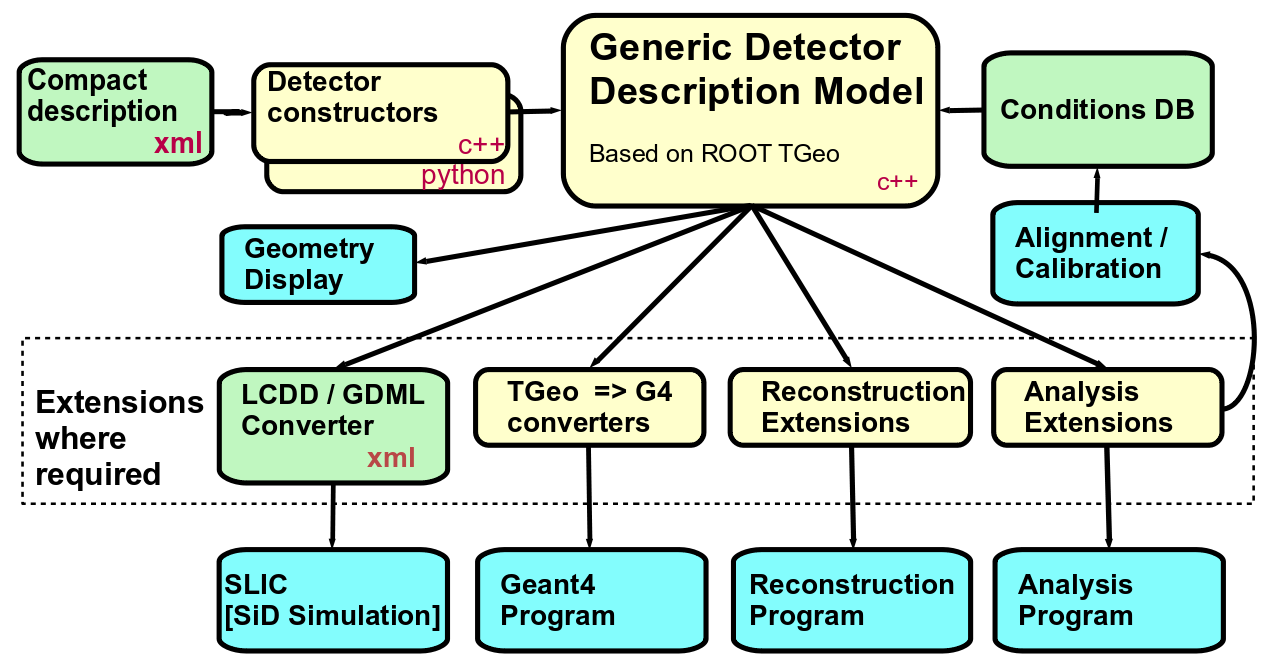
\includegraphics[width=0.8\linewidth] {DD4hep_big_picture}
    \caption{The components of the DD4hep detector geometry toolkit.}
    \label{fig:dd4hep-big-picture}
  \end{center}
  \vspace{-0.4cm}
\end{figure}


\section{Toolkit Design}
\label{sec:toolkit-design}

Figure~\ref{fig:dd4hep-big-picture} shows the architecture  of the main components of the toolkit and their interfaces  to the end-user applications, namely the simulation, reconstruction, alignment and visualization.  The central element of the toolkit is the so-called generic detector description model. This is an in-memory model, i.e., a set of \texttt{C++} objects holding the data describing the geometry and other information of the detector. The rest of the toolkit consists of tools and interfaces to input or output information from this generic detector model. The model and its components will be described in subsequence sections.

\subsection{The Compact Detector Description}
\label{sec:problem_analysis}

Inspired from the work of the linear collider detector simulation~\cite{Gaede:81331}, the compact detector description is used to define an ideal detector as typically used during the conceptual design phase of an experiment. The compact description in its minimalistic form is probably not going to be adequate later in the detector life cycle and is likely to be replaced or refined when a more realistic detector with deviations from the ideal would be needed by the experiment.

In the compact description the detector is parametrized in minimalistic terms with user provided parameters in \texttt{XML}. \texttt{XML} is an open format, the DD4hep parsers do not validate against a fix schema and hence allow to easily introduce new elements and attributes to describe detectors. This feature minimizes the burden on the end-user while still  supporting flexibility.

Such a compact detector descriptions cannot be interpreted in a general manner, therefore so called \textit{Detector Constructors} are needed.

\subsection{Detector Constructors}
\label{sec:detector-constructors}

Detector Constructors are relatively small code fragments that get as input an \texttt{XML} element from the compact description that represents  a single detector instance. The code interprets the data and expands  its geometry model in memory using the elements from the generic detector description model described in section~\ref{subsec:generic-model}. The toolkit invokes these code fragments in a data driven way using naming conventions during the initialization phase of the  application. Users focus on one single detector type at the time, but the toolkit supports them to still construct complex and large detector setups. Two implementations are currently supported: One is based on \texttt{C++}, which performs better and is able to detect errors at compiler time, but the code is slightly more technical. The other is based on Python fragments, the code is more readable and compact but errors are only detected at execution time.


The compact description together with the detector constructors are sufficient to build the detector model and to visualize it. If during the lifetime of the experiment the detector model changes, the corresponding constructors will need to be adapted accordingly. DD4hep provides already a palette of basic pre-implemented geometrical detector concepts to design experiments. In view of usage of DD4hep as a detector  description toolkit, this library may in the future also adopt generic designs of detector components created by end users e.g. during the design  phase of future experiments.

\begin{figure}[t]
  \begin{center}
    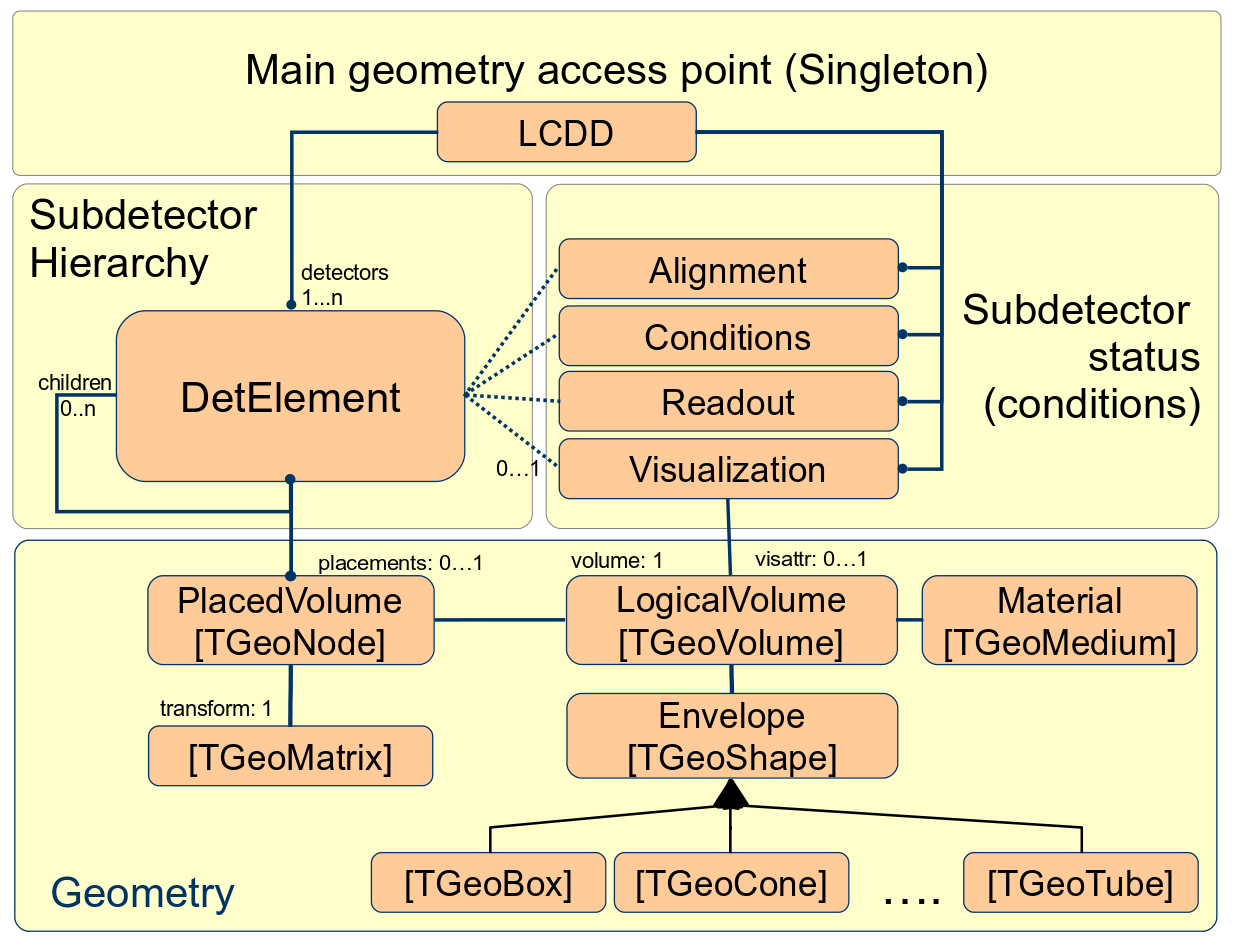
\includegraphics[width=0.8\linewidth]{DD4hep_classes}
    \caption{Class diagram with the main classes and their relations 
             for the Generic Detector Description Model. The implementing
             ROOT classes are shown in brackets.}
    \label{fig:dd4hep-detector-model}
  \end{center}
\end{figure}


\section{Generic Detector Description Model}
\label{subsec:generic-model}

This is the heart of the DD4hep detector description toolkit. Its purpose is  to build in memory a model of the detector including its geometrical aspects as well as structural and functional aspects. The design reuses the elements from the ROOT geometry package and extends them in case required functionality is not available. Figure~\ref{fig:dd4hep-detector-model} illustrates the main players and their relationships. Any detector is modeled as a tree of \textit{Detector Elements}, the entity  central to this design, which is represented in the implementation by  the \texttt{DetElement} class~\cite{Antunes-Nobrega:630827}. It offers all applications a natural entry point to any detector part of the experiment and represents a complete sub-detector (e.g. TPC), a part of a  sub-detector (e.g. TPC-Endcap), a detector module or any other convenient detector device.  The main purpose is to give access to the data associated to the detector device. For example, if the user writes some TPC reconstruction code, accessing the TPC detector element from this code will provide access  the all TPC geometrical dimensions, the alignment and calibration constants  and other slow varying conditions such as the gas pressure, end-plate  temperatures etc. The \textit{Detector Element} acts as a data concentrator. Applications may access the full experiment geometry and all connected data through a singleton object called \texttt{Detector}, which provides  management, bookkeeping and ownership to the model instances.

The geometry is implemented using the ROOT geometry classes, which are used directly without unnecessary interfaces to isolate the end-user from the  actual ROOT based implementation. There is one exception: The constructors are wrapped to facilitate a very compact and readable notation to end-users building custom \textit{Detector Constructors}.

\subsection{Detector Element Tree versus the Geometry Hierarchy}
\label{subsect:detelement-hierarchy}

The geometry part of the detector description is delegated to the ROOT classes. \textit{Logical Volumes} are the basic objects used in building the geometrical hierarchy.  A \textit{Logical Volume} is a shape with its dimensions and consist of a given material. 
They represent unpositioned objects which store all information about  the placement of possibly embedded volumes. The same volume can be replicated several times in the geometry. The \textit{Logical Volume} also  represents a system of reference with respect to its containing volumes. The reuse of instances of \textit{Logical Volumes} for different placements  optimizes the memory consumption and detailed geometries for complex setups consisting of millions of volumes may be realized with reasonable amount of memory. The difficulty is to identify a given positioned volume  in space and e.g. applying misalignment to one of these volumes. The relationship between the Detector Element and the placements is not defined by a single reference to the placement, but the full path from the top of the detector geometry model to resolve existing ambiguities due to the reuse of \textit{Logical Volumes}. Hence, individual volumes must be identified by their full path from mother to daughter starting from the top-level volume. 

\begin{figure}[t]
  \begin{center}
    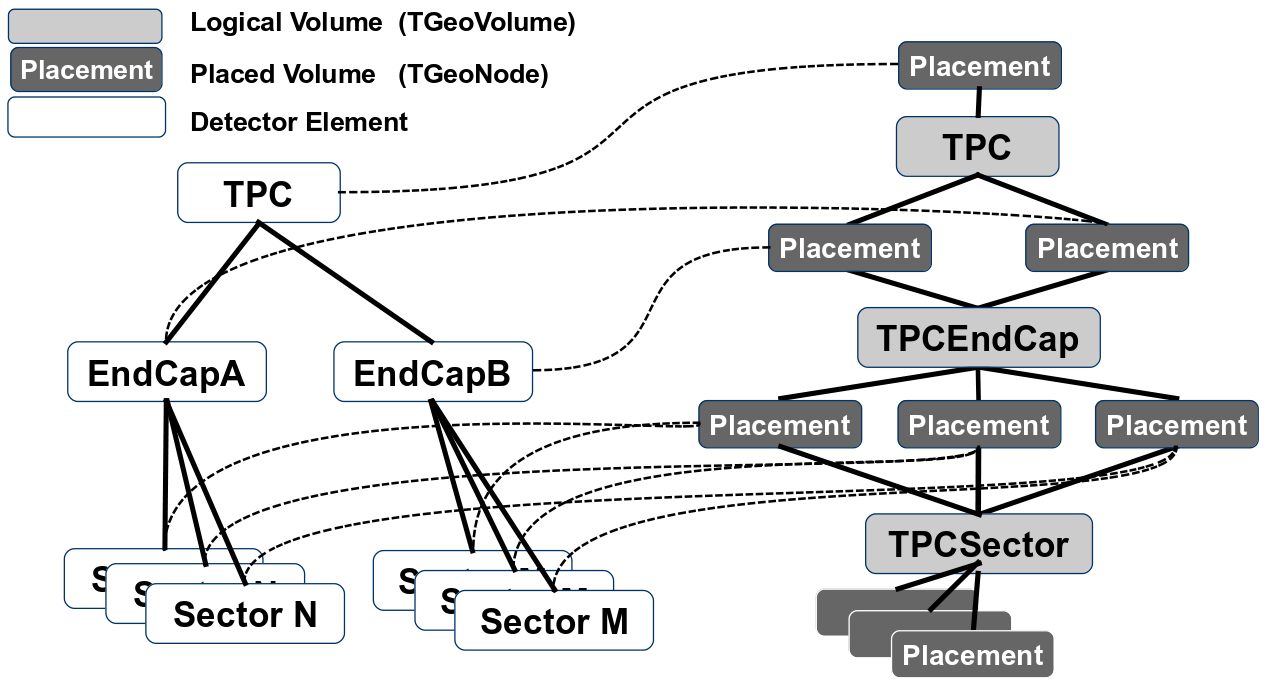
\includegraphics[width=0.8\linewidth] {DD4hep_detelement_tree}
    \caption{The object diagram of a hypothetical TPC detector showing in
    parallel the \textit{Detector Element} and the \textit{Geometry} hierarchy and the 
    relationships between the objects.}
    \label{fig:dd4hep-hierarchies}
  \end{center}
\end{figure}

The tree structure of Detector Elements is a parallel structure to the geometrical hierarchy. This structure will probably not be as deep as the geometrical one since there would not need to associate detector information at very fine-grain 
level - it is unlikely that every little metallic screw needs associated detector information such as alignment, conditions, etc. Though this screw and many other replicas must be described in the geometry  description since it may be important e.g. for its material contribution  in the simulation application. Thus, the tree of Detector Elements is fully degenerate and each detector element object will be placed only  once in the detector element tree as illustrated for a hypothetical TPC detector in Figure~\ref{fig:dd4hep-hierarchies}.

\subsection{Extensions and Views}
\label{subsect:extesions-and-views}

As depicted in Figure~\ref{fig:dd4hep-big-picture} the reconstruction application will require special functionality extending the basics  offered by the common detector element. This functionality may be implemented by a set of specialized classes that will extend the  detector element. These extensions will be in charge  of providing specific answers to the questions formulated by the  reconstruction algorithms such as pattern recognition, tracking, vertexing, particle identification, etc. One example could be to transform a calorimeter  cell identifier into a 3D space position in the global coordinate system. A generic detector description toolkit would be unable to answer this concrete question, however it provides a convenient  environment for the developer to slot-in code fragments, which implement the additional functionality using parameters stored in the \texttt{XML} compact description.

Depending on the functionality these specialized component must be able to either store additional data, expose additional behavior or both. Additional  behavior may easily be added overloading the \texttt{DetElement} class using its  internal data. The internal data is public and addressed by reference, hence any number of views extending the \texttt{DetElement} behavior may be constructed  with very small overhead. Additional data may be added by any user at any time to any instance of the \texttt{DetElement} class using a simple aggregation  mechanism shown in Figure~\ref{fig:dd4hep-extensions}. Data extensions must differ by their type. The freedom to attach virtually any data item allows for optimized attachments depending on the  application type, such as special attachments for reconstruction, simulation, tracking, etc.

\begin{figure}[t]
  \begin{center}
    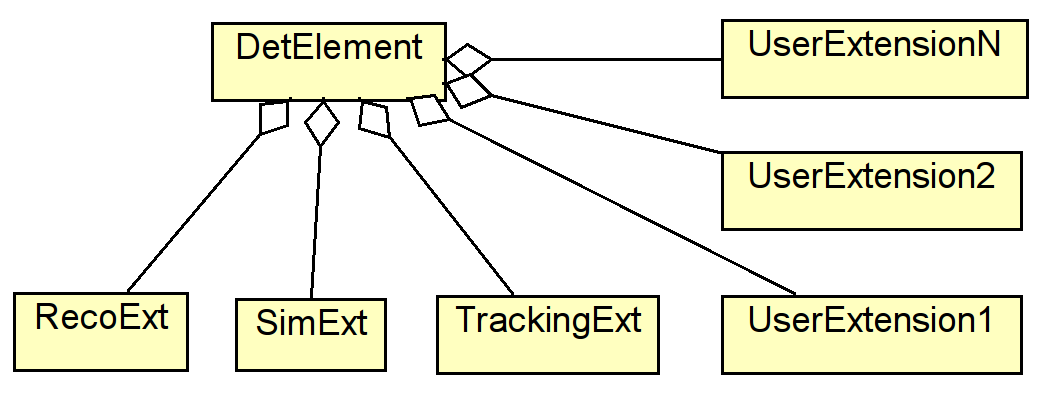
\includegraphics[width=0.8\linewidth] {DD4hep-extensions}
    \caption{Extensions may be attached to common Detector Elements which 
             extend the functionality of the common DetElement 
             class and support e.g. caching of precomputed values.}
    \label{fig:dd4hep-extensions}
  \end{center}
\end{figure}

This design allows to build views addressing the following use-cases:
\begin{description}
\item[Convenience Views] provide higher level abstractions and internally group complex calculations. Such views simplify  the life of the end-users.
\item[Optimization Views] allows end-users extend the data of the common detector detector element and store precomputed results, which would be expensive to obtain repeatedly.
\item[Compatibility Views] help to ensure smooth periods of  software redesign. During the life-time of the experiment often various software constructs are for functional reasons  re-designed and re-engineered. Compatibility Views either adapt new data designs to existing application code or expose new behavior based on existing data.
\end{description}

\section{Simulation Support}
\label{subsect:simulation-support}

Detector-simulation depends strongly on the use of an underlying simulation toolkit,  the most prominent candidate nowadays being Geant4~\cite{Agostinelli:2002hh}. DD4hep supports simulation activities with Geant4 providing an automatic translation mechanism between geometry representations. The simulation response in the active elements of the detector is not implemented by the toolkit, since it is strongly influenced by the technical choices and precise simulations depends on the very specific detection techniques. In Geant4 this response is computed in software constructs called \textit{Sensitive Detectors}.

Ideally DD4hep aims to provide a generic simulation application. Similar to the palette of pre-implemented geometrical detector  concepts to design experiments, it provides a palette of \textit{Sensitive Detectors} to simulate the detector response in form of a component library. Detector designers may base the simulation of a planned experiment  on these predefined components for initial design and optimization studies.  In a similar way easy access and configuration of other user actions of Geant4 is provided.

\section{Detector Alignment Support}
\label{subsect:alignment-support}

The support for alignment operations is crucial to the usefulness of the toolkit. In the linear collider community this support is basically missing  in all the currently used geometry description systems. The possibility to apply into the detector description alignment \textit{deltas}  (differences with respect the ideal or measured position) and read them from an external source is mandatory to exploit the toolkit. A typical alignment application would consist of calculating a new set of \textit{deltas} from a given starting point, which could then be loaded and applied again in order to validate the alignment by recalculating some alignment residuals. The ROOT geometry package supports to apply an [mis]-alignment to \textit{touchable} objects in the geometry. \textit{Touchable} objects are identified by the path of positioned volumes starting with the top node (e.g. path=\texttt{$/TOP/A_1/B_4/C_3$}). Contrary to ordinary multiple placements of \textit{Logical Volumes}, \textit{touchable} objects are degenerate and only valid for one single volume~\cite{Brun2003676}. To simplify the usage for the end user, the identification of a positioned volume will be connected to the Detector Element, where only the relative path with respect to the Detector Element will have to be specified rather the full path from the top volume. The \textit{delta}-values will have to be read from various data sources. The initial implementation will be based on simple \texttt{XML} files, later a connection to other sources such as the detector conditions database is envisaged.


\chapter{Basics}
\label{sec:dd4hep-user-manual}

This chapter describes how supply a physics application developed with all the information related to the detector which is necessary to process data from particle collisions and to qualify the detecting apparatus in order to interpret these event data.

The clients of the detector description are the algorithms residing in the  event processing framework that need this information in order to perform their job (reconstruction, simulation, etc.). The detector description provided by DD4hep is a framework for developers to provide the specific detector information to software algorithms, which process data from particle collisions.

In the following sections an overview is given over the various independent elements of DD4hep followed by the discussion of an example which leads to  the description of a detector when combining these elements. This includes a discussion of the features of the DD4hep detector description and of its structure. 

\section{Building DD4hep}
\label{sec:dd4hep-user-manual-building}

The DD4hep source code is freely available and is distributed under the GPLv3 License. See the \texttt{doc/LICENSE} in the repository~\cite{dd4hep-repo} for more information. Please read the \textit{Release Notes} before downloading or using this release.

The DD4hep project consists of several packages. The idea  has been to separate the common parts of  the detector description toolkit from concrete detector examples. 

The package {\texttt{DDCore}} contains the definition of the basic classes of the toolkit: \texttt{Handle}, \texttt{DetElement}, \texttt{Volume}, \texttt{PlacedVolume}, \texttt{Shapes}, \texttt{Material}, etc. Most of these classes are \texttt{handles} to ROOT's TGeom classes.

\subsection{Supported Platforms}
\label{sec:dd4hep-user-manual-platforms}
Actively supported and tested platforms for DD4hep are :
\begin{itemize}
\item \texttt{Scientic Linux CERN 6}
\item \texttt{CERN CentOS 7}
\item \texttt{Apple macOS}
\end{itemize}
Support for any other platform will well be taken into account, but can only be actively supported by users who submit the necessary patches.

\subsection{Prerequisites}
\label{sec:dd4hep-user-manual-prerequisites}

DD4hep depends on a number of external packages. The user will need to install these in his/her system before building and running the examples
\begin{itemize}
\item \texttt{CMake} version 3.4 or higher 
\item \texttt{ROOT 6} installations.
\item \texttt{Xerces-C} if used to parse compact descriptions an installation of {Xerces-C} will is required.
\item To build DDG4 it is mandatory to have an installation of the \texttt{Boost} header files.
\item To build and run the simulation examples \texttt{Geant4} will be required. 
\end{itemize}

\subsection{CMake Build Options for DD4hep}
\label{sec:dd4hep-user-manual-building}

The package provides the basic mechanisms for constructing the \textit{Generic Detector Description Model} in memory from \texttt{XML} compact detector definition files. Two methods are currently supported: one based
on the \texttt{C++} \texttt{Xerces-C} parser.

The \texttt{XML} parsing method is enabled by default using the \texttt{TinyXML} parser. Optionally instead of \texttt{TinyXML} the \texttt{Xerces-C}  parser may be chosen by setting the two configuration options appropriately:

\begin{minted}[frame=single,framesep=3pt,breaklines=true,tabsize=2,linenos]{shell}
    -DD4HEP_USE_XERCESC=ON
    -DXERCESC_ROOT_DIR=<path to Xerces-C-installation-directory>
\end{minted}

DDG4 is the package that contains the conversion of DD4hep geometry into Geant4 geometry to be used for simulation. The option \texttt{DD4HEP\_WITH\_GEANT4:BOOL} controls the building or not of this package that has the dependency to Geant4. The Geant4 installation needs to be located using the variable:

\begin{minted}[frame=single,framesep=3pt,breaklines=true,tabsize=2,linenos]{shell}
   -DDD4HEP_WITH_GEANT4=ON
   -DGeant4_DIR=<path to Geant4Config.cmake>
\end{minted}

To properly handle component properties using \texttt{boost::spirit}, access to the Boost header files must be provided.
\begin{minted}[frame=single,framesep=3pt,breaklines=true,tabsize=2,linenos,fontsize=\small]{bash}
    -DBoost_INCLUDE_DIR=<path to the boost include directory>
    -DBoost_NO_BOOST_CMAKE=ON  (to disable the search of boost-cmake)
\end{minted}

To build only the doxygen documentation and user manuals without the need for any dependencies one can use the following command
\begin{minted}[frame=single,framesep=3pt,breaklines=true,tabsize=2,linenos]{shell}
  cmake -DBUILD_DOCS_ONLY=ON ..
\end{minted}
After one can execute the following target for building doxygen documentaion
\begin{minted}[frame=single,framesep=3pt,breaklines=true,tabsize=2,linenos]{shell}
make reference
\end{minted}
and for building the user manuals
\begin{minted}[frame=single,framesep=3pt,breaklines=true,tabsize=2,linenos]{shell}
make pdf
\end{minted}

\subsection{Build From Source}
\label{sec:dd4hep-user-manual-building-from-source}
NEED REWRITE ONCE FINALIZED
%The following steps are necessary to build DD4hep:
%\begin{itemize}
%\item Set the environment, at least ROOT needs to be initialized, e.g.
%    \begin{minted}[frame=single,framesep=3pt,breaklines=true,tabsize=2,linenos,fontsize=\small]{bash}
%      source  /data/ilcsoft/root/5.34.03/bin/thisroot.sh
%    \end{minted}
%    \vspace{-0.6cm}
%   (the bare minimum is: \texttt{export ROOTSYS=<path to root installation>}).
%
%\item First checkout code from the repository:
%    \begin{minted}[frame=single,framesep=3pt,breaklines=true,tabsize=2,linenos,fontsize=\small]{bash}
%      svn co https://svnsrv.desy.de/public/aidasoft/DD4hep/trunk DD4hep
%    \end{minted}
%    \vspace{-0.6cm}
%
%\item We refer to the directory DD4hep as the source directory. The 
%next step is to create a directory in which to configure and run the build 
%and store the build products. This directory should not be the same as, or 
%inside, the source directory. In this guide, we create this build directory 
%alongside our source directory: 
%\begin{minted}[frame=single,framesep=3pt,breaklines=true,tabsize=2,linenos]{cmake}
%      mkdir build
%      cd build
%      cmake -DCMAKE_INSTALL_PREFIX=<dd4hep-install-pasth> <CMake-options> ../DD4hep
%      make -j 4
%      make install
%    \end{minted}
%\end{itemize}
%The CMake Variable \texttt{CMAKE\_INSTALL\_PREFIX} is used to set the install directory, 
%the directory under which the DD4hep libraries, headers and support files 
%will be installed.


\subsection{Remarks}
\label{sec:dd4hep-user-manual-remarks}
The main reference is the doxygen information of DD4hep and the ROOT documentation. Please refer to these sources for a detailed view of the capabilities of each component and/or its handle. For coherence reasons, the description of the interfaces is limited to examples which illustrate the usage of the basic components. 

\subsection{Caveat}
\label{sec:dd4hep-user-manual-caveat}
NEEDS ADDITIONAL CLARIFICATION
%The atomic units in of Geant4 are (millimeter, nanosecond and MeV and radians).
%The atomic units of ROOT-TGeo are (centimeter, seconds, GeV and degrees).
%Unfortunately the authors could not agree on a common system of units
%and mixing the two can easily result in a chaos.
%Users must be aware of this fact.

\section{DD4hep Handles}
\label{sec:dd4hep-user-manual-handles}

Handles are the means of clients accessing DD4hep detector description data. The data itself is not held by the handle itself, the handle only allows the access to the data typically held by a pointer. The template handle class (see for details the \href{https://dd4hep.web.cern.ch/dd4hep/reference/classdd4hep_1_1Handle.html}{\texttt{Handle.h}} header file) allows type safe assignment of other unrelated handles and supports standard data conversions to the underlying object in form of the raw pointer, a reference etc. The template handle class:

\begin{minted}[frame=single,framesep=3pt,breaklines=true,tabsize=2,linenos,fontsize=\small]{c++}
template <typename T> class Handle {
public:
  // Type definitions and class specific abbreviations and forward declarations
  typedef T Implementation;
  typedef Handle<Implementation> handle_t;
public:
  // Single and only data member: pointer to the underlying object
  T* m_element;
public:
  Handle() : m_element(0) { }
  Handle(T* e) : m_element(e) { }
  Handle(const Handle<T>& e) : m_element(e.m_element) { }
  template<typename Q> Handle(Q* e) : m_element((T*)e) { verifyObject(); }
  template<typename Q> Handle(const Handle<Q>& e) : m_element((T*)e.m_element) { verifyObject(); }
  Handle<T>& operator=(const Handle<T>& e) { m_element=e.m_element; return *this;}
  bool isValid() const { return 0 != m_element; }
  bool operator!() const { return 0 == m_element; }
  void clear() { m_element = 0; }
  T* operator->() const { return m_element; }
  operator T& () const { return *m_element; }
  T& operator*() const { return *m_element; }
  T* ptr() const { return m_element; }
  template <typename Q> Q* _ptr() const { return (Q*)m_element; }
  template <typename Q> Q* data() const { return (Q*)m_element; }
  template <typename Q> Q& object() const { return *(Q*)m_element; }
  const char* name() const;
};
\end{minted}
effectively works like a pointer with additional object validation during assignment and construction. Handles support direct access to the held object: either by using the 
\begin{minted}[frame=single,framesep=3pt,breaklines=true,tabsize=2,fontsize=\small]{c++}
       operator->()                        (See line 19 above)
\end{minted}
or the automatic type conversions:
\begin{minted}[frame=single,framesep=3pt,breaklines=true,tabsize=2,fontsize=\small]{c++}
      operator T& ()  const                (See line 20-21 above)
      T& operator*()  const
\end{minted}

All entities of the DD4hep detector description are exposed as handles - raw pointers should not occur in the code. The handles to these objects serve two purposes:
\begin{itemize}
\item Hold a pointer to the object and extend the functionality of a raw pointer.
\item Enable the creation of new objects using specialized constructors within sub-classes. To ensure memory integrity and avoid resource  leaks these created objects should always be stored in the detector description data hub \texttt{Detector} described in section~\ref{sec:dd4hep-user-manual-LCDD-hub}.
\end{itemize}


\section{The Data Extension Mechanism}
\label{sec:dd4hep-user-manual-data-extensions}

Data extensions are client defined \texttt{C++} objects aggregated to basic DD4hep objects. The need to introduce such data extensions results from the simple fact that no data structure can be defined without the iterative need in the long term to extend it leading to implementations, which can only satisfy a subset of possible clients. To accomplish for this fact a mechanism was put in place which allows any user to attach any supplementary information provided the information is embedded in a polymorph object with an accessible destructor. There is one limitation though: object extension must differ by their interface type. There may not be two objects attached with the identical interface type. The actual implemented sub-type of the extension is not relevant. Separating the interface type from the implementation type keeps client code still functional even if the implementation of the extension changes 
or is a plug-able component.

The following code snippet shows the extension interface:

\begin{minted}[frame=single,framesep=3pt,breaklines=true,tabsize=2,linenos,fontsize=\small]{c++}
  /// Extend the object with an arbitrary structure accessible by the type
  template <typename IFACE, typename CONCRETE> IFACE* addExtension(CONCRETE* c);
  /// Access extension element by the type
  template <class T> T* extension() const;
\end{minted}

Assuming a client class of the following structure:
\begin{minted}[frame=single,framesep=3pt,breaklines=true,tabsize=2,linenos,fontsize=\small]{c++}
  class ExtensionInterface {
    virtual ~ExtensionInterface();
    virtual void foo() = 0;
  };

  class ExtensionImplementation : public ExtensionInterface {
    ExtensionImplementation();
    virtual ~ExtensionImplementation();
  virtual void foo();
  };
\end{minted}
is then attached to an extensible object as follows:
\begin{minted}[frame=single,framesep=3pt,breaklines=true,tabsize=2,linenos,fontsize=\small]{c++}
  ExtensionImplementation* ptr = new ExtensionImplementation();
  /// ... fill the ExtensionImplementation instance with data ...
  module.addExtension<ExtensionInterface>(ptr);
\end{minted}
The data extension may then be retrieved whenever the instance of the extensible object ``module'' is accessible:
\begin{minted}[frame=single,framesep=3pt,breaklines=true,tabsize=2,linenos,fontsize=\small]{c++}
  ExtensionInterface* ptr = module.extension<ExtensionInterface>();
\end{minted}
The lookup mechanism is rather efficient. Though it is advisable to cache the pointer within the client code if the usage is very frequent.

There are currently three object types present which support this mechanism:
\begin{itemize}
\item the central object of DD4hep, the \texttt{Detector} class discussed in section~\ref{sec:dd4hep-user-manual-LCDD-hub}.
\item the object describing subdetectors or parts thereof, the \texttt{DetElement} class discussed in section~\ref{sec:dd4hep-user-manual-detector-elements}. Detector element extensions in addition require the presence of a copy constructor to support e.g. reflection operations. Without a copy mechanism detector element hierarchies could cloned.
\item the object describing sensitive detectors, the \texttt{SensitiveDetector} class discussed in section~\ref{sec:dd4hep-user-manual-sensitive-detectors}.
\end{itemize}

\section{XML Tools and Interfaces}
\label{sec:dd4hep-user-manual-xml-tools}

Using native tools to interpret \texttt{XML} structures is rather tedious and lengthy. To easy the access to \texttt{XML} data considerable effort was put in place to easy the life of clients as much as possible using predefined instructs to access \texttt{XML} attributes, elements or element collections.

The functionality of the \texttt{XML} tools is perhaps best shown with a small example. Imagine to extract the data from an \texttt{XML} snippet like the following:
\begin{minted}[frame=single,framesep=3pt,breaklines=true,tabsize=2,linenos,fontsize=\small]{xml}
  <detector name="Sometthing">
    <tubs rmin="BP_radius - BP_thickness" rmax="BP_radius" zhalf="Endcap_zmax/2.0"/>
    <position x="0" y="0" z="Endcap_zmax/2.0" />
    <rotation x="0.0" y="CrossingAngle/2.0" z="0.0" />
    <layer id="1" inner_r="Barrel_r1" outer_r="Barrel_r1 + 0.02*cm" inner_z="Barrel_zmax + 0.1*cm">
      <slice material = "G10" thickness ="0.5*cm"/>
    </layer>
    <layer id="2" inner_r="Barrel_r2" outer_r="Barrel_r2 + 0.02*cm" inner_z="Barrel_zmax + 0.1*cm">
     <slice material = "G10" thickness ="0.5*cm"/>
    </layer>
    ....
  </detector>
\end{minted}

The variable names used in the \texttt{XML} snippet are evaluated when interpreted. Unless the attributes are accessed as strings, the client never sees the strings, but only the evaluated numbers. The anatomy of the \texttt{C++} code snippets to interpret such a data section looks very similar:
\begin{minted}[frame=single,framesep=3pt,breaklines=true,tabsize=2,linenos,fontsize=\small]{c++}
  static void some_xml_handler(xml_h e)  {
    xml_det_t  x_det  (e);
    xml_comp_t x_tube    = x_det.tubs();
    xml_dim_t  pos       = x_det.position();
    xml_dim_t  rot       = x_det.rotation();
    string     name      = x_det.nameStr();
      
    for(xml_coll_t i(x_det,_U(layer)); i; ++i)  {
      xml_comp_t x_layer = i;
      double  zmin = x_layer.inner_z();
      double  rmin = x_layer.inner_r();
      double  rmax = x_layer.outer_r();
      double  layerWidh = 0;
        
      for(xml_coll_t j(x_layer,_U(slice)); j; ++j)  {
        double thickness = xml_comp_t(j).thickness();
        layerWidth += thickness;
      }
    }
  }
\end{minted}
In the above code snippet an \texttt{XML} (sub-)tree is passed to the executing function as a handle to an \texttt{XML} element ({\texttt{xml\_h}}). Such handles may seamlessly be assigned to any supporting helper class inheriting from the class {\texttt{XML::Element}}, which encapsulates the functionality required to interpret the \texttt{XML} structures. Effectively the various \texttt{XML} attributes and child nodes are accessed using functions with the same name from a convenience handle. In lines 3-5 child nodes are extracted, lines 10-12,16 access element attributes.Element collections with the same tag names \texttt{layer} and \texttt{slice} are exposed to the client code using an iteration mechanism.

Note the macros $\texttt{\_U(layer)}$ and $\texttt{\_U(slice)}$:  When using \texttt{Xerces-C} as an \texttt{XML} parser, it will expand to the reference to an object containing the unicode value of the string ``layer''. The full list of predefined tag names can be found in the include file \texttt{XML/UnicodeValues.h}. If a user tag is not part in the precompiled tag list, the corresponding Unicode string may be created with the macro \texttt{\_Unicode(layer)} or the function \texttt{Unicode(``layer'')}.

The convenience handles actually implement these functions to ease life. There is no magic - newly created attributes with new names obviously cannot be accessed with convenience mechanism. Hence, either you know what you are doing and you create your own convenience handlers or you restrict yourself a bit in the creativity of defining new attribute names.

There exist several utility classes to extract data from predefined \texttt{XML} tags:
\begin{itemize}
\item Any \texttt{XML} element is described by an \texttt{XML} handle \texttt{\texttt{XML::Handle\_t}} ({\texttt{xml\_t}}). Handles are the basic structure for the support of higher level interfaces described above. The assignment of a handle to any of the interfaces below is possible.
\item The class \texttt{\texttt{XML::Element}} ({\texttt{xml\_elt\_t}}) supports in a simple way the navigation through the hierarchy of the \texttt{XML} tree accessing child nodes and attributes. Attributes at this level are named entities and the tag name must be supplied.
\item The class \texttt{\texttt{XML::Dimension}} with the type definition {\texttt{xml\_dim\_t}}, supports numerous access functions named identical to the
\texttt{XML} attribute names. Such helper classes simplify the tedious string handling required by the 
\item The class \texttt{\texttt{XML::Component}} ({\texttt{xml\_comp\_t}}) and the class \texttt{\texttt{XML::Detector}} ({\texttt{xml\_det\_t}}) resolving other issues useful to construct detectors.
\item Sequences of \texttt{XML} elements with an identical tag name may be handled as iterations as shown in the Figure above using the class \texttt{\texttt{XML::Collection\_t}}.
\item Convenience classes, which allow easy access to element attributes  may easily be constructed using the methods of the {\texttt{XML::Element}} class. This allows to construct very flexible thou non-intrusive extensions to DD4hep. Hence there is a priori no need to modify these helpers for the benefit of only one single client. In the presence of multiple requests such extensions may though be adopted.
\end{itemize}
It is clearly the responsibility of the client to only request attributes from an \texttt{XML} element, which exist. If an attribute, a child node etc. is not found within the element an exception is thrown.

The basic interface of the \texttt{XML::Element} class allows to access tags and child nodes not exposed by the convenience wrappers:
\begin{minted}[frame=single,framesep=3pt,breaklines=true,tabsize=2,linenos,fontsize=\small]{c++}
  /// Access the tag name of this DOM element
  std::string tag() const;
  /// Access the tag name of this DOM element
  const XmlChar* tagName() const;

  /// Check for the existence of a named attribute
  bool hasAttr(const XmlChar* name) const;
  /// Retrieve a collection of all attributes of this DOM element
  std::vector<Attribute> attributes() const;
  /// Access single attribute by it's name
  Attribute getAttr(const XmlChar* name) const;
  /// Access attribute with implicit return type conversion
  template <class T> T attr(const XmlChar* tag) const;
  /// Access attribute name (throws exception if not present)
  const XmlChar* attr_name(const Attribute attr) const;
  /// Access attribute value by the attribute  (throws exception if not present)
  const XmlChar* attr_value(const Attribute attr) const;

  /// Check the existence of a child with a given tag name
  bool hasChild(const XmlChar* tag) const;
  /// Access child by tag name. Thow an exception if required in case the child is not present
  Handle_t child(const Strng_t& tag, bool except = true) const;
  /// Add a new child to the DOM node
  Handle_t addChild(const XmlChar* tag) const;
  /// Check if a child with the required tag exists - if not create it and add it to the current node
  Handle_t setChild(const XmlChar* tag) const;
\end{minted}

\section{The Detector Description Data Hub: \texttt{Detector}}
\label{sec:dd4hep-user-manual-LCDD-hub}
As shown in Figure~\ref{fig:dd4hep-detector-model}, any access to the detector  description data is done using a standardized interface called \texttt{Detector}. During the configuration phase of the detector the interface is used to populate the internal data structures. Data structures present in the memory layout of the detector description may be retrieved by clients at any time using the  \href{https://dd4hep.web.cern.ch/dd4hep/reference/classdd4hep_1_1Detector.html}{\texttt{Detector} interface class}. This includes of course, the access during the actual detector construction. The following code listing shows the accessor method to retrieve  detector description entities from the interface. Not shown are access methods for groups of these entities and the methods to add objects:

\begin{minted}[frame=single,framesep=3pt,breaklines=true,tabsize=2,linenos,fontsize=\small]{c++}
class Detector {
  ///+++ Shortcuts to access often used quantities

  /// Return handle to material describing air
  virtual Material air() const = 0;
  /// Return handle to material describing vacuum
  virtual Material vacuum() const = 0;
  /// Return handle to "invisible" visualization attributes
  virtual VisAttr invisible() const = 0;

  ///+++ Access to the top level detector elements and the corresponding volumes

  /// Return reference to the top-most (world) detector element
  virtual DetElement world() const = 0;
  /// Return reference to detector element with all tracker devices.
  virtual DetElement trackers() const = 0;

  /// Return handle to the world volume containing everything
  virtual Volume worldVolume() const = 0;
  /// Return handle to the volume containing the tracking devices
  virtual Volume trackingVolume() const = 0;

  ///+++ Access to geometry and detector description objects

  /// Retrieve a constant by it's name from the detector description
  virtual Constant constant(const std::string& name)      const = 0;
  /// Retrieve a matrial by it's name from the detector description
  virtual Material material(const std::string& name)      const = 0;
  /// Retrieve a field component by it's name from the detector description
  virtual DetElement detector(const std::string& name)      const = 0;
  /// Retrieve a sensitive detector by it's name from the detector description
  virtual SensitiveDetector sensitiveDetector(const std::string& name) const = 0;
  /// Retrieve a readout object by it's name from the detector description
  virtual Readout readout(const std::string& name)       const = 0;
  /// Retrieve a id descriptor by it's name from the detector description
  virtual IDDescriptor idSpecification(const std::string& name)   const = 0;
  /// Retrieve a subdetector element by it's name from the detector description
  virtual CartesianFieldfield(const std::string& name)     const = 0;

  ///+++ Access to visualisation attributes and Geant4 processing hints

  /// Retrieve a visualization attribute by it's name from the detector description
  virtual VisAttr visAttributes(const std::string& name) const = 0;

  /// Retrieve a region object by it's name from the detector description
  virtual Region  region(const std::string& name)    const = 0;
  /// Retrieve a limitset by it's name from the detector description
  virtual LimitSet limitSet(const std::string& name)      const = 0;
  //...
  
  ///+++ Extension mechanism:
  /// Extend the sensitive detector element with an arbitrary structure accessible by the type
  template <typename IFACE, typename CONCRETE> IFACE* addExtension(CONCRETE* c)
};
\end{minted}

As shown in the above listing, the \texttt{Detector} interface is the main access point to access a whole set 
\begin{itemize}
\item often used predefined values such as the material ``air'' or ``vacuum'' (line 5--10).
\item the top level objects ``world'', ``trackers'' and the corresponding volumes (line 14--21).
\item items in the constants table containing named definitions also used during the interpretation of the \texttt{XML} content after parsing (line 26)
\item named items in the the material table (line 28)
\item named subdetectors after construction and the corresponding (line 30)
\item named sensitive detectors with their (line 32)
\item named readout structure definition using a (line 34)
\item named readout identifier descriptions (line 36)
\item named descriptors of electric and/or magnetic fields  (line 39).
\end{itemize}
Additional support for specialized applications is provided by the interface:
\begin{itemize}
\item Geant4: named region settings  (line 46)
\item Geant4: named limits settings  (line 48)
\item Visualization: named visualization attributes  (line 43)
\item User defined extensions (line 53) are supported with the extension mechanism described in section~\ref{sec:dd4hep-user-manual-data-extensions}.
\end{itemize}

All the values are populated either directly from \texttt{XML} or from \textit{detector constructors} (see section~\ref{sec:detector-constructors}). The interface also allows to load \texttt{XML} configuration files of any kind provided an appropriate  interpretation plugin is present. In the next section we describe the functionality  of the ``lccd'' plugin used to interpret the compact detector description. This mechanism can easily be extended using ROOT plugins, where the plugin name must corrspond to the \texttt{XML} root element of the document to be interpreted.

\section{Detector Description Persistency in \texttt{XML}}
\label{sec:compact-xml-structure}
As explained in a previous section, the mechanism involved in the data loading  allow an application to be fairly independent of the technology used to populate the transient detector representation. However, if one wants to use a given technology, she/he has to get/provide the corresponding conversion mechanism. The choice of \texttt{XML} was driven mainly by its easiness of use and the number of tools provided for its manipulation and parsing. Moreover, \texttt{XML} data can be easily translated into many other format using tools like \texttt{XSLT}  processors. The grammar used for the \texttt{XML} data is pretty simple and straight forward, actually very similar to other geometry description languages based on \texttt{XML}. For example the material description is nearly identical to the material description in \texttt{GDML}~\cite{Chytracek:2006be}. The syntactic structure of the compact \texttt{XML} description was taken from the SiD detector description~\cite{Gaede:81331}. The following listing shows the basic layout of any the compact detector description file with its different sections:

\begin{minted}[frame=single,framesep=3pt,breaklines=true,tabsize=2,linenos,fontsize=\small]{xml}
<lccdd>
  <info>   ...    </info>       Auxiliary detector model information
  <includes>  ... </includes>   Section defining GDML files to be included
  <define>  ...   </define>     Dictionary of constant expressions and varables
  <materials> ... </materials>  Additional material definitions
  <display>  ...  </display>    Definition of visualization attributes
  <detectors> ... </detectors>  Section with sub-detector definitions
  <readouts>  ... </readouts>   Section with readout structure definitions
  <limits>  ...   </limits>     Definition of limit sets for Geant4
  <fields>  ...   </fields>     Field definitions
</lccdd>
\end{minted}

The root tag of the \texttt{XML} tree is {\texttt{lccdd}}. This name is fixed. In the following the content of the various sections is discussed. The \texttt{XML} sections are filled with the following information:
\begin{itemize}
\item {\textbf{The \texttt{<info>} sub-tree}} contains auxiliary information about the detector model:
\begin{minted}[frame=single,framesep=3pt,breaklines=true,tabsize=2,linenos,fontsize=\small]{xml}
<info name="clic_sid_cdr"
  title="CLIC Silicon Detector CDR"
  author="Christian Grefe"
  url="https://twiki.cern.ch/twiki/bin/view/CLIC/ClicSidCdr"
  status="development"
  version="$Id: compact.xml 665 2013-07-02 18:49:26Z markus.frank $">
  <comment>The compact format for the CLIC Silicon Detector used 
           for the conceptual design report</comment>
</info>
\end{minted}

\item {\textbf{The \texttt{<includes>} section}} allows to include GDML sub-trees containing material descriptions. These files are processed {\textit{before}} the detector constructors are called:
\begin{minted}[frame=single,framesep=3pt,breaklines=true,tabsize=2,linenos,fontsize=\small]{xml}
<includes>
  <gdmlFile  ref="elements.xml"/>
  <gdmlFile  ref="materials.xml"/>
   ...
</includes>
\end{minted}

\item {\textbf{The \texttt{<define>} section}} contains all variable definitions defined by the client to simplify the definition of subdetectors. These name-value pairs are fed to the expression evaluator and must evaluate to a number. String constants are not allowed. These variables can be combined to formulas e.g. to automatically re-dimension subdetectors if boundaries are changed:
\begin{minted}[frame=single,framesep=3pt,breaklines=true,tabsize=2,linenos,fontsize=\small]{xml}
<define>
  <constant name="world_side" value="30000"/>
  <constant name="world_x" value="world_side"/>
  <constant name="world_y" value="world_side"/>
  <constant name="world_z" value="world_side"/>
  ....
</define>
\end{minted}

\item  {\textbf{The \texttt{<materials>} sub-tree}} contains additional materials, which are not contained in the default materials tables. The snippet below shows an example to extend the table of known materials. For more details please see section~\ref{sec:compact-material-description}.
\begin{minted}[frame=single,framesep=3pt,breaklines=true,tabsize=2,linenos,fontsize=\small]{xml}
<materials>
  <!-- The description of an atomic element or isotope -->
  <element Z="30" formula="Zn" name="Zn" >
    <atom type="A" unit="g/mol" value="65.3955" />
  </element>
  ...
  <!-- The description of a new material               -->
  <material name="CarbonFiber_15percent">
    ...
  </material>
  ...
</materials>
\end{minted}

\item {\textbf{The visualization attributes}} are defined in the \texttt{<display>} section. Clients access visualization settings by name. The possible attributes are shown below and essentially contain the RGB color values, the visibility and the drawing style:
\begin{minted}[frame=single,framesep=3pt,breaklines=true,tabsize=2,linenos,fontsize=\small]{xml}
<display>
  <vis name="InvisibleNoDaughters"      
       showDaughters="false" 
       visible="false"/>
  <vis name="SiVertexBarrelModuleVis" 
       alpha="1.0" r="1" g="1" b="0.6" 
       drawingStyle="solid" 
       showDaughters="true" 
       visible="true"/>
  ....
</display>
\end{minted}

\item {\textbf{<Limisets>}} contain parameters passed to Geant4:
\begin{minted}[frame=single,framesep=3pt,breaklines=true,tabsize=2,linenos,fontsize=\small]{xml}
<limits>
    <limitset name="cal_limits">
        <limit name="step_length_max" particles="*" value="5.0" unit="mm" />
    </limitset>
</limits>
\end{minted}

\item {\textbf{The \texttt{detectors}}} section contains subtrees of the type \texttt{<detector>} which contain all parameters used by the \textit{detector constructors} to actually expand the geometrical structure. Each subdetector has a name and a type, where the type is used to call the proper constructor plugin. If the subdetector element is sensitive, a forward reference to the corresponding readout structure is mandatory. The remaining parameters are user defined:

\begin{minted}[frame=single,framesep=3pt,breaklines=true,tabsize=2,linenos,fontsize=\small]{xml}
<detectors>
  <detector id="4" name="SiTrackerEndcap" type="SiTrackerEndcap" readout="SiTrackerEndcapHits">
    <comment>Outer Tracker Endcaps</comment>
    <module name="Module1" vis="SiTrackerEndcapModuleVis">
      <trd x1="36.112" x2="46.635" z="100.114/2" />
      <module_component thickness="0.00052*cm"   material="Copper" />
      <module_component thickness="0.03*cm"   material="Silicon" sensitive="true" />
      ...
    </module> 
    ...
    <layer id="1">
      <ring r="256.716" zstart="787.105+1.75" nmodules="24" dz="1.75" module="Module1"/>
      <ring r="353.991" zstart="778.776+1.75" nmodules="32" dz="1.75" module="Module1"/>
      <ring r="449.180" zstart="770.544+1.75" nmodules="40" dz="1.75" module="Module1"/>
    </layer>
    ...
  </detector>
</detectors>
\end{minted}

\item {\textbf{The \texttt{<readouts>} section}} defined the encoding of sensitive volumes to so-called cell-ids, which are in DD4hep 64-bit integer numbers. The encoding is subdetector dependent with one exception: to uniquely identity each subdetector, the width of the system field must be the same.
\begin{minted}[frame=single,framesep=3pt,breaklines=true,tabsize=2,linenos,fontsize=\small]{xml}
<readouts>
  <readout name="SiTrackerEndcapHits">
    <id>system:8,barrel:3,layer:4,module:14,sensor:2,side:32:-2,strip:20</id>
  </readout>
  ...
</readouts>
\end{minted}

\item {\textbf{Electromagnetic fields}} are described in the \texttt{<fields>} section. There may be several fields present. In DD4hep the resulting field vectors
may be both electric and magnetic. The strength of the overall field is calculated as the superposition of the individual components:
\begin{minted}[frame=single,framesep=3pt,breaklines=true,tabsize=2,linenos,fontsize=\small]{xml}
<fields>
  <field name="GlobalSolenoid" type="solenoid" 
         inner_field="5.0*tesla"
         outer_field="-1.5*tesla" 
         zmax="SolenoidCoilOuterZ"
         outer_radius="SolenoidalFieldRadius">
  </field>
  ...
</fields>
\end{minted}
\end{itemize}

\section{Material Description}
\label{sec:compact-material-description}

Materials are needed by logical volumes. They are defined as isotopes,  elements or mixtures. Elements can optionally be composed of isotopes. Composition is always done by specifying the fraction of the mass. Mixtures can be composed of elements or other mixtures. For a mixture the user can specify composition either by number of atoms or by fraction of mass. The materials sub-tree in section~\ref{sec:compact-xml-structure} shows the representation of an element, a simple material and a  composite material in the \texttt{XML} format identical to GDML~\cite{Chytracek:2006be}. The snippet below shows how to define new material instances:
\begin{minted}[frame=single,framesep=3pt,breaklines=true,tabsize=2,linenos,fontsize=\small]{xml}
<materials>
  ...
  <!-- (1) The description of an atomic element or isotope -->
  <element Z="30" formula="Zn" name="Zn" >
    <atom type="A" unit="g/mol" value="65.3955" />
  </element>
  <!-- (2) A composite material                            -->
  <material name="Kapton">
    <D value="1.43" unit="g/cm3" />
    <composite n="22" ref="C"/>
    <composite n="10" ref="H" />
    <composite n="2" ref="N" />
    <composite n="5" ref="O" />
  </material>
  <!-- (3) A material mixture                              -->
  <material name="PyrexGlass">
    <D type="density" value="2.23" unit="g/cm3"/>
    <fraction n="0.806" ref="SiliconOxide"/>
    <fraction n="0.130" ref="BoronOxide"/>
    <fraction n="0.040" ref="SodiumOxide"/>
    <fraction n="0.023" ref="AluminumOxide"/>
  </material>
  ...
</materials>
\end{minted}

The \texttt{<materials>} sub-tree contains additional materials, which are not contained in the default materials tables. The snippet above shows different kinds of materials:
\begin{itemize}
\item[1.] Atomic elements as they are in the periodic table. The number of elements is finite. It is unlikely any client will have to extend the known elements.
\item[2.] Composite materials, which consists of one or several elements forming a molecule. These materials have a certain density under normal conditions described in the child element \texttt{D}.
For each \texttt{composite} the attribute \texttt{ref} denotes the element type by name,  the attribute \texttt{n} denotes the atomic multiplicity.  Typically each of the elements in (1) also forms such a material representing objects which consist of pure material like e.g. iron magnet yokes or copper wires.
\item[3.] Last there are mixtures of composite materials to describe  for example alloys, solutions or other mixtures of solid materials. This is the type of material used to actually create mechanical structures forming the assembly of an experiment. Depending on the manufacturing these materials have a certain density (\texttt{D}) and are composed of numerous molecules contributing to the resulting material with a given \texttt{fraction}. The sum of all fractions (attribute \texttt{n}) is 1.0.
\end{itemize}
``Real'' materials i.e. those you can actually touch are described in TGeo by the class \texttt{TGeoMedium}.
\footnote{Typical beginner's mistake: Do not mix up the  two classes \texttt{TGeoMaterial} and \texttt{TGeoMedium}! The material to define volumes is of type \texttt{TGeoMedium}, which also includes the 
description of the material's finish.}. Materials are not constructed by any client. Materials and elements are  either already present in the the corresponding tables of the ROOT geometry package or they are added during the interpretation of the \texttt{XML} input. Clients access the description of material using the \texttt{Detector} interface.

\begin{figure}[t]
  \begin{center}
    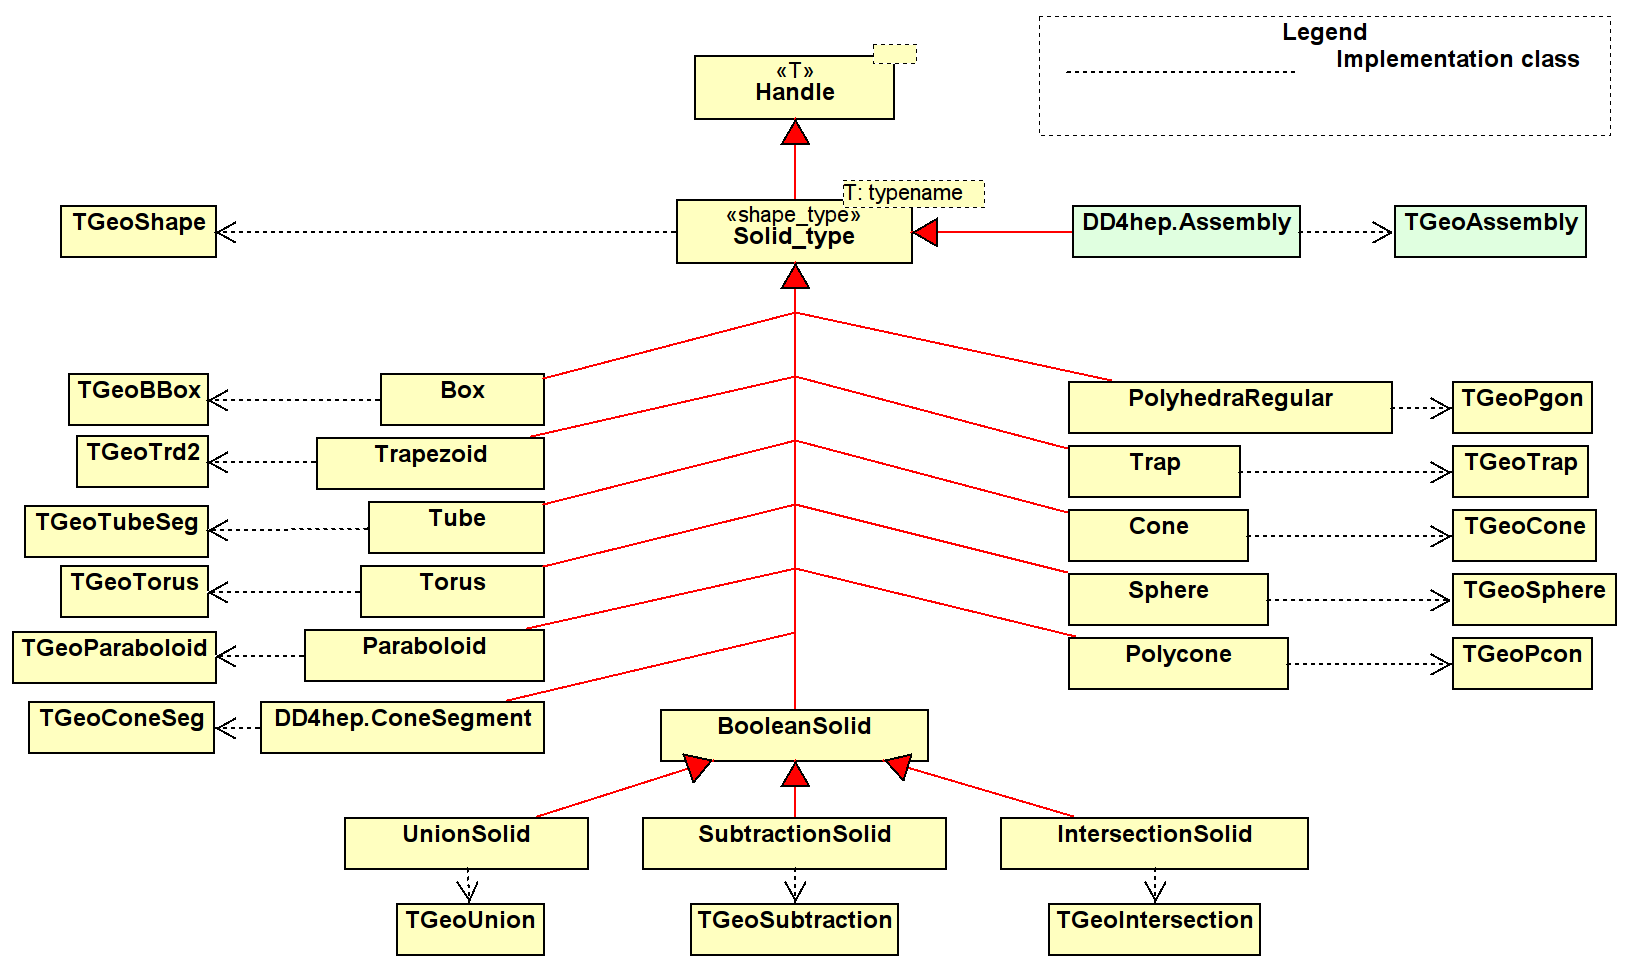
\includegraphics[width=160mm] {DD4hep-solids}
    \caption{Extensions may be attached to common Detector Elements which 
             extend the functionality of the common DetElement 
             class and support e.g. caching of precomputed values.}
    \label{fig:dd4hep-solids}
  \end{center}
  \vspace{-0.6cm}
\end{figure}

\section{Shapes}
\label{dd4hep-basic-shapes}

Shapes are abstract objects with a bounding surface and fixed dimensions.  There are primitive, atomic shapes and complex boolean shapes as shown in Figure~\ref{fig:dd4hep-solids}.  TGeo and similarly Geant4 offer a whole palette of primitive shapes, which can be used to construct more complex shapes:
\begin{itemize}
\item \texttt{Box} shape represented by the \texttt{TGeoBBox} class. To create a new box object call one of the following constructors:
\begin{minted}[frame=single,framesep=3pt,breaklines=true,tabsize=2,linenos,fontsize=\small]{c++}
/// Constructor to be used when creating an anonymous new box object
Box(double x, double y, double z);
/// Constructor to be used when creating an anonymous new box object
template<typename X, typename Y, typename Z> Box(const X& x, const Y& y, const Z& z);
\end{minted}
\item \texttt{Sphere} shape represented by the \texttt{TGeoSphere} class. To create a new sphere object call one of the following constructors:
\item \texttt{Cone}  shape represented by the \texttt{TGeoCone} class. To create a new cone object call one of the following constructors:
\begin{minted}[frame=single,framesep=3pt,breaklines=true,tabsize=2,linenos,fontsize=\small]{c++}
/// Constructor to create a new anonymous object with attribute initialization
Cone(double z,double rmin1,double rmax1,double rmin2,double rmax2);
template<typename Z, typename RMIN1, typename RMAX1, typename RMIN2, typename RMAX2>
Cone(const Z& z, const RMIN1& rmin1, const RMAX1& rmax1, const RMIN2& rmin2, const RMAX2& rmax2);
\end{minted}
\item \texttt{ConeSegment} shape represented by the \texttt{TGeoConeSeg} class. To create a new cone segment object call one of the following constructors:
\begin{minted}[frame=single,framesep=3pt,breaklines=true,tabsize=2,linenos,fontsize=\small]{c++}
/// Constructor to create a new ConeSegment
ConeSegment(double dz, double rmin1, double rmax1, double rmin2, double rmax2, double phi1=0.0, double phi2=2.0*M_PI);
\end{minted}
\item \texttt{Polycone} shape represented by the \texttt{TGeoPcon} class. To create a new polycone object call one of the following constructors:
\begin{minted}[frame=single,framesep=3pt,breaklines=true,tabsize=2,linenos,fontsize=\small]{c++}
/// Constructor to create a new polycone object
Polycone(double start, double delta);
followed by a call to:
void addZPlanes(const std::vector<double>& rmin, 
                const std::vector<double>& rmax,
                const std::vector<double>& z);
/// Constructor to create a new polycone object. Add at the same time all Z planes
Polycone(double start, double delta, 
         const std::vector<double>& rmin, 
         const std::vector<double>& rmax, 
         const std::vector<double>& z);
\end{minted}
\item \texttt{TubeSegment} shape represented by the \tgeo{TGeoTubeSeg}{\texttt TGeoTubeSeg} class. To create a new tube segment object call one of the following constructors:
\begin{minted}[frame=single,framesep=3pt,breaklines=true,tabsize=2,linenos,fontsize=\small]{c++}
Tube(double rmin, double rmax, double z, double deltaPhi=2*M_PI)
Tube(double rmin, double rmax, double z, double startPhi, double deltaPhi)

template<typename RMIN, typename RMAX, typename Z, typename DELTAPHI>
Tube(const RMIN& rmin, const RMAX& rmax, const Z& z, const DELTAPHI& deltaPhi)  

template<typename RMIN, typename RMAX, typename Z, typename STARTPHI, typename DELTAPHI>
Tube(const std::string& name, const RMIN& rmin, const RMAX& rmax, const Z& z, 
     const STARTPHI& startPhi, const DELTAPHI& deltaPhi)  
\end{minted}
\item \texttt{Trapezoid} shape represented by the \texttt{TGeoTrd} class. To create a new trapezoid object call one of the following constructors:
\begin{minted}[frame=single,framesep=3pt,breaklines=true,tabsize=2,linenos,fontsize=\small]{c++}
/// Constructor to create a new anonymous object with attribute initialization
Trapezoid(double x1, double x2, double y1, double y2, double z);
\end{minted}
\item \texttt{Trap} shape represented by the \tgeo{TGeoTrap}{\texttt TGeoTrap} class. To create a new trap object call one of the following constructors:
\begin{minted}[frame=single,framesep=3pt,breaklines=true,tabsize=2,linenos,fontsize=\small]{c++}
/// Constructor to create a new anonymous object with attribute initialization
Trap(double z,double theta,double phi,
     double y1,double x1,double x2,double alpha1,
     double y2,double x3,double x4,double alpha2);
/// Constructor to create a new anonymous object for right angular wedge from STEP (Se G4 manual for details)
Trap( double pz, double py, double px, double pLTX);
\end{minted}
\item \texttt{Torus}  shape represented by the \tgeo{TGeoTorus}{\texttt TGeoTorus} class. To create a new torus object call one of the following constructors:
\begin{minted}[frame=single,framesep=3pt,breaklines=true,tabsize=2,linenos,fontsize=\small]{c++}
/// Constructor to create a new anonymous object with attribute initialization
Torus(double r, double rmin, double rmax, double phi=M_PI, double delta_phi=2.*M_PI);
\end{minted}
\item \texttt{Paraboloid}  shape represented by the \tgeo{TGeoParaboloid}{\texttt TGeoParaboloid} class. To create a new paraboloid object call one of the following constructors:
\begin{minted}[frame=single,framesep=3pt,breaklines=true,tabsize=2,linenos,fontsize=\small]{c++}
/// Constructor to create a new anonymous object with attribute initialization
Paraboloid(double r_low, double r_high, double delta_z);
\end{minted}
\item \texttt{PolyhedraRegular} shape represented by the \texttt{TGeoPgon} class. To create a new polyhedron object call one of the following constructors:
\begin{minted}[frame=single,framesep=3pt,breaklines=true,tabsize=2,linenos,fontsize=\small]{c++}
/// Constructor to create a new object. Phi(start)=0, deltaPhi=2PI, Z-planes at +-zlen/2
PolyhedraRegular(int nsides, double rmin, double rmax, double zlen);
/// Constructor to create a new object. Phi(start)=0, deltaPhi=2PI, Z-planes at zplanes[0],[1]
PolyhedraRegular(int nsides, double rmin, double rmax, double zplanes[2]);
/// Constructor to create a new object with phi_start, deltaPhi=2PI, Z-planes at +-zlen/2
PolyhedraRegular(int nsides, double phi_start, double rmin, double rmax, double zlen);
\end{minted}
\end{itemize}

Besides the primitive shapes three types of boolean shapes (described in TGeo by the \texttt{TGeoCompositeShape} class) are supported:

\begin{itemize}
\item \texttt{UnionSolid} objects representing the union,
\item \texttt{IntersectionSolid} objects representing the intersection,
\item \texttt{SubtractionSolid} objects representing the subtraction,
\end{itemize}

of two other primitive or complex shapes. To build a boolean shape, the second shape is transformed in 3-dimensional space before the boolean operation is applied. The 3D transformations are described by objects from the \texttt{ROOT::Math} library and are supplied at construction time.  Such a transformation as shown in the code snippet below may be 

\begin{itemize}
\item The identity transformation. Then no transformation object needs to be provided (see line 2).
\item A translation only described by a \texttt{Position} object (see line 4)
\item A 3-fold rotation first around the Z-axis, then around the Y-axis and finally around the X-axis. For transformation operations of this kind a \texttt{RotationZYX} object must be supplied (see line 6).
\item A generic 3D rotation matrix should be applied to the second shape. Then a \texttt{Rotation3D} object must be supplied (see line 8).
\item Finally a generic 3D transformation (translation+rotation) may be applied using a \texttt{Transform3D} object (see line 10).
\end{itemize}

All three boolean shapes have constructors as shown here for the \texttt{UnionSolid}:
\begin{minted}[frame=single,framesep=3pt,breaklines=true,tabsize=2,linenos,fontsize=\small]{c++}
  /// Constructor to create a new object. Position is identity, Rotation is identity-rotation!
  UnionSolid(const Solid& shape1, const Solid& shape2);
  /// Constructor to create a new object. Placement by position, Rotation is identity-rotation!
  UnionSolid(const Solid& shape1, const Solid& shape2, const Position& pos);
  /// Constructor to create a new object. Placement by a RotationZYX within the mother
  UnionSolid(const Solid& shape1, const Solid& shape2, const RotationZYX& rot);
  /// Constructor to create a new object. Placement by a generic rotoation within the mother
  UnionSolid(const Solid& shape1, const Solid& shape2, const Rotation3D& rot);
  /// Constructor to create a new object. Placement by a generic transformation within the mother
  UnionSolid(const Solid& shape1, const Solid& shape2, const Transform3D& pos);
\end{minted}

\subsection{Shape factories} 
Sometimes it is useful to create shapes in an ``abstract'' way e.g. to define areas in the detector. To create such shapes a factory method was implemented, which allows to create a valid shape handle given a valid \texttt{XML} element providing the required attributes. The factory methods are invoked using from \texttt{XML} elements of the following form:
\begin{minted}[frame=single,framesep=3pt,breaklines=true,tabsize=2,linenos,fontsize=\small]{xml}
  <some_element type="shape-type" .... args ....>
\end{minted}

The shape is then constructed using the \texttt{XML} component object:
\begin{minted}[frame=single,framesep=3pt,breaklines=true,tabsize=2,linenos,fontsize=\small]{c++}
#include "XML/Helper.h"

xml_h e = <shape-element>;
Box box = xml_comp_t(e).createShape();
if ( !box.isValid() ) { /* ...handle error ... */  }
\end{minted}
The required arguments for the various shapes are then:
\begin{itemize}
\item For a Box:
\begin{minted}[frame=single,framesep=3pt,breaklines=true,tabsize=2,linenos,fontsize=\small]{xml}
  <some_element type="Box" x="x-value" y="y-value" z="z-value"/>
\end{minted}
fulfilling a constructor of the type: \texttt{Box(dim.dx(), dim.dy(), dim.dz())}.

\item For a Polycone:
\vspace{-0.2cm}
\begin{minted}[frame=single,framesep=3pt,breaklines=true,tabsize=2,linenos,fontsize=\small]{xml}
  <some_element type="Polycone" start="start-phi-value" deltaphi="delta-phi-value">
    <zplane z="z-value" rmin="rmin-value" rmax="rmax-value"/>
    <zplane z="z-value" rmin="rmin-value" rmax="rmax-value"/>
    .... any number of Z-planes ....
    <zplane z="z-value" rmin="rmin-value" rmax="rmax-value"/>
  </some_element>
\end{minted}

\item For a ConeSegment the following constructor must be fulfilled: 
\begin{minted}[frame=single,framesep=3pt,breaklines=true,tabsize=2,linenos,fontsize=\small]{c++}
ConeSegment(e.rmin(0.0), e.rmax(), e.z(0.0), e.startphi(0.0), e.deltaphi(2*M_PI))}
\end{minted}
where the above default values for the \texttt{XML} attributes \texttt{rmin}, \texttt{z}, \texttt{startphi} and \texttt{deltaphi} are used if not explicitly stated in the \texttt{XML} element \texttt{e}.

\item For a Tube the constructor is:
\begin{minted}[frame=single,framesep=3pt,breaklines=true,tabsize=2,linenos,fontsize=\small]{c++}
Tube(e.rmin(0.0), e.rmax(), e.z(0.0), e.startphi(0.0), e.deltaphi(2*M_PI))
\end{minted}

\item For a Cone the constructor is:
\begin{minted}[frame=single,framesep=3pt,breaklines=true,tabsize=2,linenos,fontsize=\small]{c++}
double rmi1 = e.rmin1(0.0), rma1 = e.rmax1();
Cone(e.z(0.0), rmi1, rma1, e.rmin2(rmi1), e.rmax2(rma1))
\end{minted}

\item For a Trap the constructor is: if \texttt{dz} is specified: 
\begin{minted}[frame=single,framesep=3pt,breaklines=true,tabsize=2,linenos,fontsize=\small]{c++}
Trap(e.dz(), e.dy(), e.dx(),_toDouble(_Unicode(pLTX)))
\end{minted}
Otherwise: 
\begin{minted}[frame=single,framesep=3pt,breaklines=true,tabsize=2,linenos,fontsize=\small]{c++}
Trap(e.z(0.0), e.theta(), e.phi(0), e.y1(), e.x1(), e.x2(), e.alpha(), e.y2(), e.x3(), e.x4(), e.alpha2())
\end{minted}
\item For a Trapezoid the constructor is:
\begin{minted}[frame=single,framesep=3pt,breaklines=true,tabsize=2,linenos,fontsize=\small]{c++}
Trapezoid(e.x1(), e.x2(), e.y1(), e.y2(), e.z(0.0))
\end{minted}
\item For a Torus the constructor is:
\begin{minted}[frame=single,framesep=3pt,breaklines=true,tabsize=2,linenos,fontsize=\small]{c++}
Torus(e.r(), e.rmin(), e.rmax(), e.phi(M_PI), e.deltaphi(2.*M_PI))
\end{minted}
\item For a Sphere the constructor is:
\begin{minted}[frame=single,framesep=3pt,breaklines=true,tabsize=2,linenos,fontsize=\small]{c++}
Sphere(e.rmin(), e.rmax(), e.deltatheta(M_PI), e.phi(0e0),e.deltaphi(2.*M_PI))
\end{minted}
\item For a Paraboloid the constructor is:
\begin{minted}[frame=single,framesep=3pt,breaklines=true,tabsize=2,linenos,fontsize=\small]{c++}
Paraboloid(e.rmin(0.0), e.rmax(), e.dz())
\end{minted}
\item For a PolyhedraRegular the constructor is:
\begin{minted}[frame=single,framesep=3pt,breaklines=true,tabsize=2,linenos,fontsize=\small]{c++}
PolyhedraRegular(e.numsides(), e.rmin(), e.rmax(), e.dz())
\end{minted}
\end{itemize}

\section{Volumes and Placements}

The detector geometry is described by a hierarchy of volumes and their  corresponding placements. Both, the TGeo package and Geant4~\cite{Agostinelli:2002hh} are following effectively the same ideas ensuring an easy conversion from TGeo to Geant4 objects for the simulation application. A volume is an unplaced solid de\-scribed in terms of a primitive shape or a boolean operation of solids, a material and a number of placed sub-volumes (placed volumes) inside. The class diagram showing the relationships between volumes and placements, solids and materials is shown in Figure~\ref{fig:dd4hep-detector-model}.
It is worth noting, that any volume has children, but no parent or ``mother'' volume. This is a direct consequence of the requirement to re-use volumes and place the same volume arbitrarily often. Only the act of placing a volume defines the relationship to the next level parent volume. The resulting geometry tree is very effective, simple and convenient to  describe the detector geometry hierarchy starting from the top level volume representing e.g. the experiment cavern down to the very detail of the detector e.g. the small screw in the calorimeter. The top level volume is the very only volume without a placement. All geometry calculations, computations are always  performed within the local coordinate system of the volume. The following example code shows how to create a volume which consists of a given material and with a shape. The created volume is then placed inside the mother-volume using the local coordinate system of the mother volume:

\begin{minted}[frame=single,framesep=3pt,breaklines=true,tabsize=2,linenos,fontsize=\small]{c++}
  Volume       mother = ....ampercent

  Material     mat    (lcdd.material("Iron"));
  Tube         tub    (rmin, rmax, zhalf);
  Volume       vol    (name, tub, mat);
  Transform3D  tr     (RotationZYX(rotz,roty,rotx),Position(x,y,z));
  PlacedVolume phv = mother.placeVolume(vol,tr);
\end{minted}

The volume has the shape of a tube and consists of iron. Before being placed, the daughter volume is transformed within the mother coordinate system according to the requested transformation. The example also illustrates how to access \texttt{Material} objects from the \texttt{Detector} interface.

The {\texttt{Volume}} class provides several possibilities to declare the required space transformation necessary to place a daughter volume  within the mother:
\begin{itemize}
\item to place a daughter volume unrotated at the origin of the mother, the 
transformation is the identity. Use the following call to place the daughter:
\begin{minted}[frame=single,framesep=3pt,breaklines=true,tabsize=2,linenos,fontsize=\small]{c++}
PlacedVolume placeVolume(const Volume& vol)  const;
\end{minted}
\item If the positioning is described by a simple translation, use:
\begin{minted}[frame=single,framesep=3pt,breaklines=true,tabsize=2,linenos,fontsize=\small]{c++}
PlacedVolume placeVolume(const Volume& vol, const Position& pos)  coampercentnst;
\end{minted}
\item In case the daughter should be rotated first around the Z-axis, then around the Y-axis and finally around the X-axis place the daughter using this call:
\begin{minted}[frame=single,framesep=3pt,breaklines=true,tabsize=2,linenos,fontsize=\small]{c++}
PlacedVolume placeVolume(const Volume& vol, const RotationZYX& rot)  const;
\end{minted}
\item If the full 3-dimensional rotation matrix is known use:
\begin{minted}[frame=single,framesep=3pt,breaklines=true,tabsize=2,linenos,fontsize=\small]{c++}
PlacedVolume placeVolume(const Volume& vol, const Rotation3D& rot)  const;
\end{minted}
\item for an entirely unconstrained placement place the daughter providing a \texttt{Transform3D} object:
\begin{minted}[frame=single,framesep=3pt,breaklines=true,tabsize=2,linenos,fontsize=\small]{c++}
PlacedVolume placeVolume(const Volume& volume, const Transform3D& tr)  const;
\end{minted}
\end{itemize}

For more details of the \texttt{Volume} and the \texttt{PlacedVolume} classes please see the header file \texttt{Volumes.h}.

One volume like construct is special: the assembly constructs. Assemblies are volumes without shapes. The ``assembly'' shape does not own a own surface by itself, but rather defines it's surface and 
bounding box from the contained children. In this corner also the implementation concepts between TGeo and Geant4 diverge. Whereas TGeo handles assemblies very similar to real volumes, in Geant4 assemblies are purely artificial and disappear at the very moment volumes  are placed.

\section{Detector Elements}
\label{sec:dd4hep-user-manual-detector-elements}

\begin{figure}[b]
  \begin{center}
    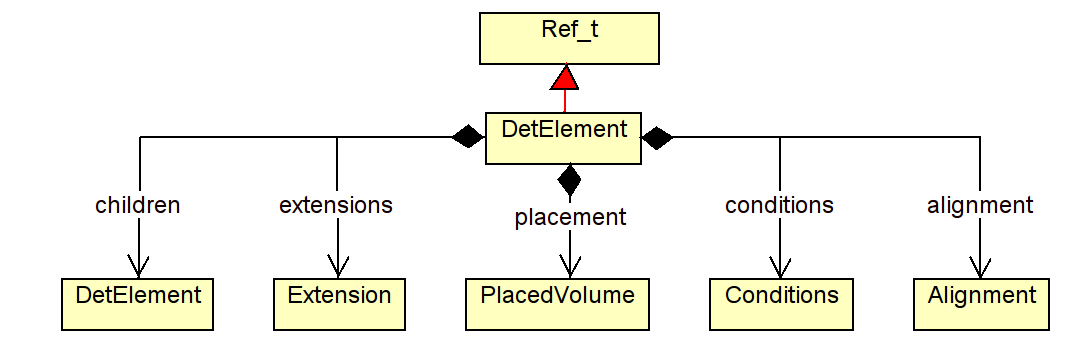
\includegraphics[width=160mm] {DD4hep-detelement-drawing}
    \caption{The basic layout of the \texttt{DetElement} class aggregating
        all data entities necessary to process data.}
    \label{fig:dd4hep-user-manual-detelement-drawing}
  \end{center}
  \vspace{-0.6cm}
\end{figure}

Detector elements (class \texttt{DetElement}) are entities which represent  subdetectors or sizable parts of a subdetector. As shown in Figure~\ref{fig:dd4hep-user-manual-detelement-drawing}, a \texttt{DetElement} instance has the means to provide to clients information about

\begin{itemize}
\item generic properties like the detector type or the path within the \texttt{DetElement}s hierarchy:
\begin{minted}[frame=single,framesep=3pt,breaklines=true,tabsize=2,linenos,fontsize=\small]{c++}
  /// Access detector type (structure, tracker, calorimeter, etc.).
  std::string type() const;
  /// Path of the detector element (not necessarily identical to placement path!)
  std::string path() const;
\end{minted}

\item the detector hierarchy by exposing its children. The hierarchy may be  accessed with the following API:
\begin{minted}[frame=single,framesep=3pt,breaklines=true,tabsize=2,linenos,fontsize=\small]{c++}
  /// Add new child to the detector structure
  DetElement& add(DetElement sub_element);
  /// Access to the list of children
  const Children& children() const;
  /// Access to individual children by name
  DetElement child(const std::string& name) const;
  /// Access to the detector elements's parent
  DetElement parent() const;
\end{minted}

\item its placement within the overall experiment if it represents an entire subdetector or its placement with respect to its parent if the \texttt{DetElement} represents a part of a subdetector. The placement path is the fully qualified path of placed volumes  from the top level volume to the placed detector element. % and may serve as a shortcut for the eqnarrayment implementation:
\begin{minted}[frame=single,framesep=3pt,breaklines=true,tabsize=2,linenos,fontsize=\small]{c++}
  /// Access to the full path to the placed object
  std::string placementPath() const;
  /// Access to the physical volume of this detector element
  PlacedVolume placement() const;
  /// Access to the logical volume of the daughter placement
  Volume volume() const;
\end{minted}

\item information about the environmental conditions etc. (\texttt{conditons}):
\begin{minted}[frame=single,framesep=3pt,breaklines=true,tabsize=2,linenos,fontsize=\small]{c++}
  /// Access to the conditions information 
  Conditions conditions() const;
\end{minted}

%\item eqnarrayment information:
%\begin{minted}[frame=single,framesep=3pt,breaklines=true,tabsize=2,linenos,fontsize=\small]{c++}
%  /// Access to the eqnarrayment information
%  eqnarrayment eqnarrayment() const;
%\end{minted}

\item convenience information such as cached transformations to/from the top level volume, to/from the parent \texttt{DetElement} and to/from another \texttt{DetElement} in the hierarchy above:
\begin{minted}[frame=single,framesep=3pt,breaklines=true,tabsize=2,linenos,fontsize=\small]{c++}
  /// Transformation from local coordinates of the placed volume to the world system
  bool localToWorld(const Position& local, Position& global) const;
  /// Transformation from world coordinates of the local placed volume coordinates
  bool worldToLocal(const Position& global, Position& local) const;

  /// Transformation from local coordinates of the placed volume to the parent system
  bool localToParent(const Position& local, Position& parent) const;
  /// Transformation from world coordinates of the local placed volume coordinates
  bool parentToLocal(const Position& parent, Position& local) const;

  /// Transformation from local coordinates of the placed volume to arbitrary parent system set as reference
  bool localToReference(const Position& local, Position& reference) const;
  /// Transformation from world coordinates of the local placed volume coordinates
  bool referenceToLocal(const Position& reference, Position& local) const;

  /// Set detector element for reference transformations. 
  /// Will delete existing reference transformation.
  DetElement& setReference(DetElement reference);
\end{minted}

\item User extension information as described in section~\ref{sec:dd4hep-user-manual-data-extensions}:
\begin{minted}[frame=single,framesep=3pt,breaklines=true,tabsize=2,linenos,fontsize=\small]{c++}
  /// Extend the detector element with an arbitrary structure accessible by the type
  template <typename IFACE, typename CONCRETE> IFACE* addExtension(CONCRETE* c);
  /// Access extension element by the type
  template <class T> T* extension() const;
\end{minted}

\end{itemize}

\section{Sensitive Detectors}
\label{sec:dd4hep-user-manual-sensitive-detectors}

Though the concept of sensitive detectors comes from Geant4 and simulation  activities, in DD4hep the sensitive detectors are the client interface to  access the readout description (class \texttt{Readout}) with its  segmentation of sensitive elements (class \texttt{Segmentation}) and the description of hit decoders (class \texttt{IDDescriptors}). As shown in Figure~\ref{fig:dd4hep-sensitive-detectors}, these object instances are required when reconstructing data from particle collisions.

Besides the access to data necessary for reconstruction the sensitive detector also hosts Region setting (class \texttt{Region} and sets of cut limits (class \texttt{LimitSets}) used to configure the Geant4 simulation toolkit. The following code snippet shows the accessors of the  \texttt{SensitiveDetector} class to obtain the corresponding  information~\footnote{The methods to set the data are not shown here.}:

\begin{minted}[frame=single,framesep=3pt,breaklines=true,tabsize=2,linenos,fontsize=\small]{c++}
    struct SensitiveDetector: public Ref_t {
      /// Access the hits collection name
      const std::string& hitsCollection() const;
      /// Access readout structure of the sensitive detector
      Readout readout() const;
      /// Access to the region setting of the sensitive detector (not mandatory)
      Region region() const;
      /// Access to the limit set of the sensitive detector (not mandatory).
      LimitSet limits() const;

      /// Extend the sensitive detector element with an arbitrary structure accessible by the type
      template <typename IFACE, typename CONCRETE> IFACE* addExtension(CONCRETE* c);
      /// Access extension element by the type
      template <class T> T* extension() const;
   };
\end{minted}

\begin{figure}[h]
  \begin{center}
    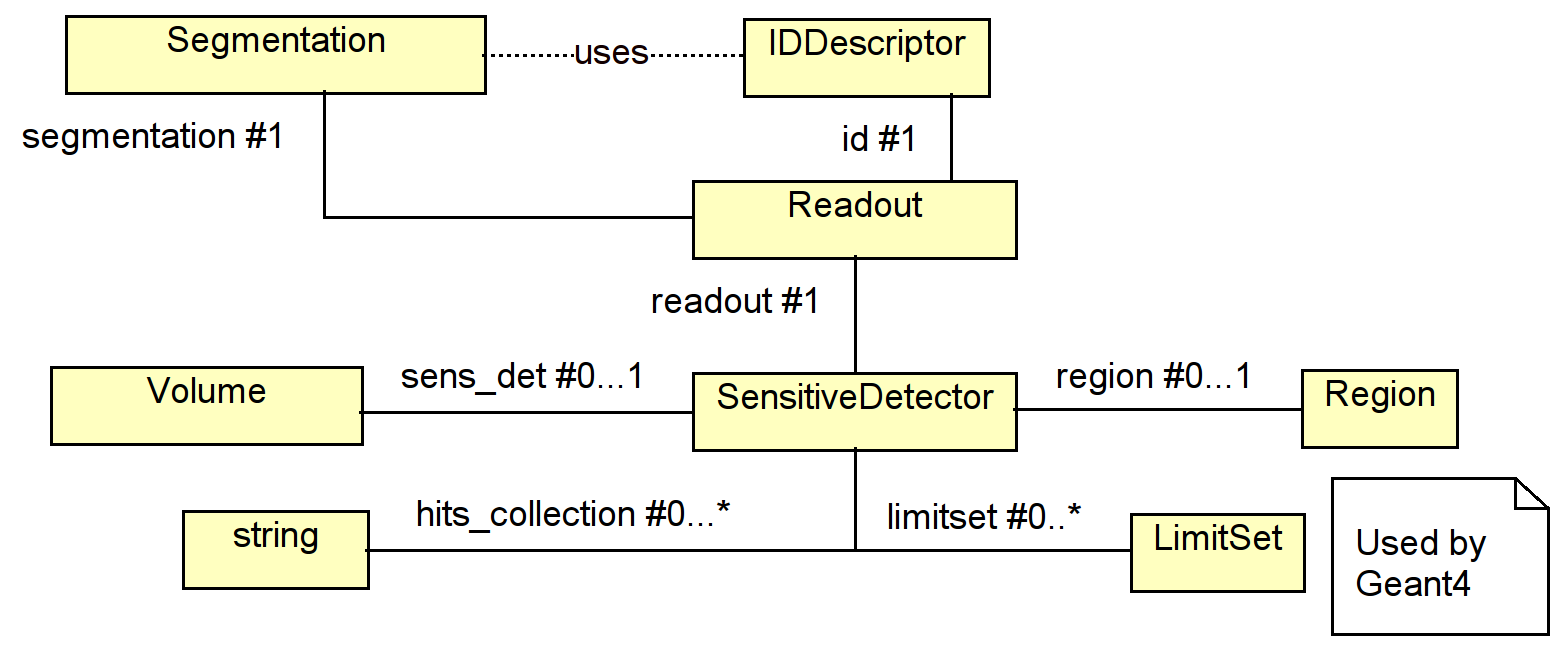
\includegraphics[width=140mm] {DD4hep-sensitive-detectors}
    \caption{The structure of DD4hep sensitive detectors.}
    \label{fig:dd4hep-sensitive-detectors}
  \end{center}
  \vspace{-0.6cm}
\end{figure}

Sensitive detector objects are automatically creating using the information of the \texttt{<readout>} section of the \texttt{XML} file if a subdetector is sensitive and references a valid readout entry. In the detector constructor (or any time later) clients  may add additional information to a sensitive detector object using  an extension mechanism similar to the extension mechanism for  detector elements mentioned earlier.

Volumes may be shared and reused in several placements. In the parallel hierarchy of detector elements as shown in Figure~\ref{fig:dd4hep-hierarchies}, the detector elements may reference unambiguously the volumes of their respective placements, but not the reverse. However, the sensitive detector setup is a single instance per subdetector. Hence it may be referenced by all sensitive Volumes of one subdetector. In the following chapters the access to the readout structure is described.

\section{Description of the Readout Structure}
\label{sec:dd4hep-manual-readout-description}

The \texttt{Readout} class describes the detailed structure of a sensitve volume. The for example may be the layout of strips or pixels in a silicon detector i.e. the description of entities which would not be modeled using individual volumes and placements though this would theoretically  feasible. Each sensitive element is segmented according to the \texttt{Segmentation} object and hits resulting from energy depositions in the sensitive volume are  encoded using the \texttt{IDDescriptor} object.

\begin{figure}[h]
  \begin{center}
    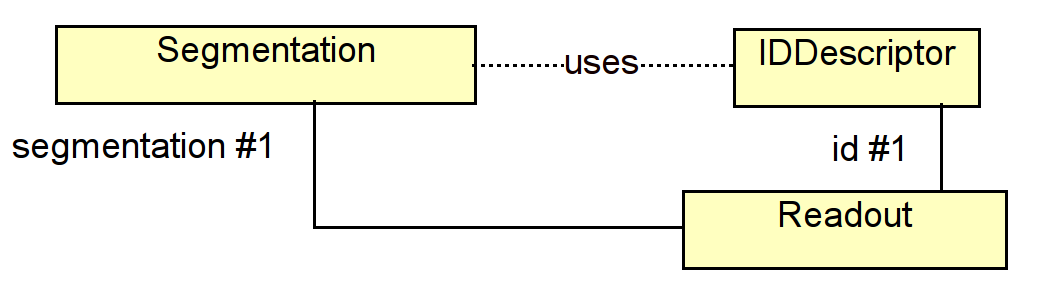
\includegraphics[width=100mm] {DD4hep-readout}
    \caption{The basic components to describe the \texttt{Readout} structure
    of a subdetector. }
    \label{fig:dd4hep-sensitive-detectors}
  \end{center}
  \vspace{-0.6cm}
\end{figure}

\subsection{CellID Descriptors}
\label{sec:dd4hep-manual-readout-iddescriptors}

\texttt{IDDescriptor}s define the encoding of sensitive volumes to uniquely identify the location of the detector response. The encoding defines a bit-field with the length of 64 bits. The first field is mandatory called \texttt{system} and identifies the subdetector. All other fields define the other volumes in the hierarchy. The high bits are not necessarily mapped to small daughter volumes, but may simply identify a logical segmentation such as the \texttt{strip} \texttt{number} within a wafer of a vertex detector as shown in the following \texttt{XML} snippet: 
\begin{minted}[frame=single,framesep=3pt,breaklines=true,tabsize=2,linenos,fontsize=\small]{xml}
<readouts>
  <readout name="SiVertexEndcapHits">
    <id>system:8,barrel:3,layer:4,module:14,sensor:2,side:32:-2,strip:24</id>
  </readout>
<readouts>
\end{minted}
These identifiers are the data input to  \texttt{segmentation classes}~\ref{sec:dd4hep-manual-readout-segmentations}, which define a user friendly API to en/decode the detector response.

\subsection{Segmentations}
\label{sec:dd4hep-manual-readout-segmentations}

Segementations define the user API to the low level interpretation of the energy deposits in a subdetector. For technical reasons and partial religious reasons are the segmentation implementation not part of the DD4hep  toolkit, but an independent package call \texttt{DDSegmentation}. Though the usage is an integral part of DD4hep.

\subsection{Volume Manager}
The \texttt{VolumeManager} is a tool to seek a lookup table of placements of  sensitive volumes and their corresponding unique volume identifier, the \texttt{cellID}. The volume manager analyzes - once the geometry is closed - the hierarchical tree and stores the various placements in the hierarchy with respect to their identifiers. In other words the the tree is  reused volumes shown e.g. in Figure~\ref{fig:dd4hep-hierarchies} is degenerated  according to the full pathes of the various volumes. This  use case is very common to reconstruction and analysis applications whenever a given raw-data (aka ``hit'') element must be related to its geometrical location.

Figure~\ref{fig:dd4hep-user-manual-volmgr} shows the design diagram of this component:
\begin{figure}[h]
  \begin{center}
    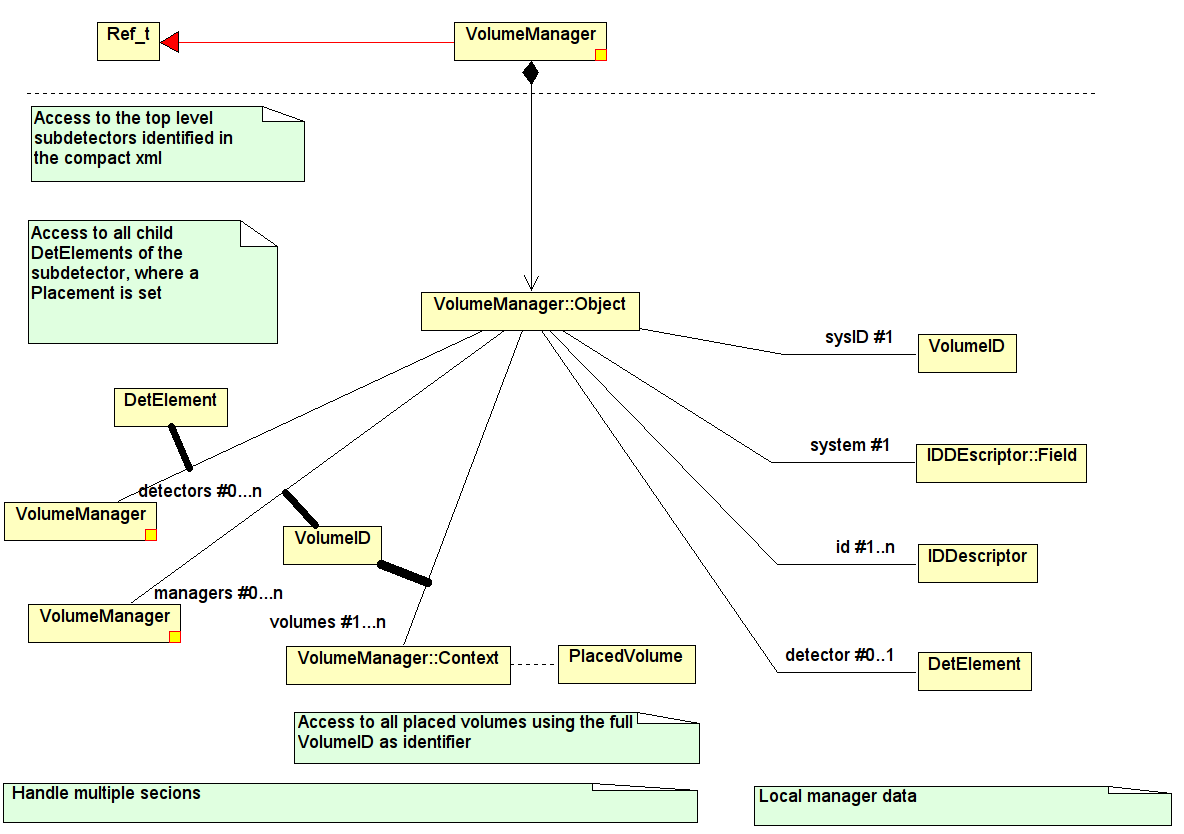
\includegraphics[width=170mm] {DD4hep-volmgr}
    \caption{Extensions may be attached to common Detector Elements which 
             extend the functionality of the common DetElement 
             class and support e.g. caching of precomputed values.}
    \label{fig:dd4hep-user-manual-volmgr}
  \end{center}
\end{figure}

To optimize the access of complex subdetector structures, is the volume-identifier map split and the volumes of each each subdetector is stored in a separate map. This optimization however is transparent to clients. The following code extract from the header files lists the main client routines to extract volume information given a known \texttt{cellID}:
\begin{minted}[frame=single,framesep=3pt,breaklines=true,tabsize=2,linenos,fontsize=\small]{c++}
  /// Lookup the context, which belongs to a registered physical volume.
  Context* lookupContext(VolumeID volume_id) const;
  /// Lookup a physical (placed) volume identified by its 64 bit hit ID
  PlacedVolume lookupPlacement(VolumeID volume_id) const;
  /// Lookup a top level subdetector detector element 
  /// according to a contained 64 bit hit ID
  DetElement lookupDetector(VolumeID volume_id) const;
  /// Lookup the closest subdetector detector element in the hierarchy 
  /// according to a contained 64 bit hit ID
  DetElement lookupDetElement(VolumeID volume_id) const;
  /// Access the transformation of a physical volume to the world coordinate system
  const TGeoMatrix& worldTransformation(VolumeID volume_id) const;
\end{minted}


\subsection{Static Electric and Magnetic Fields}
\label{sec:dd4hep-manual-static-fields}

The generic field is described by a structure of any field type (electric or magnetic) with field components in Cartesian coordinates. The overlay field is the sum of several magnetic of electric field components
and the resulting field vectors are computed by the vector addition of the individual components. The available components are described in the following. If necessary new field implementations may be added at any time: they are  instantiated when necessary by the factory mechanism. Fields are described in the compact model within the {\texttt{<fields>}} tags the following example shows:
\begin{minted}[frame=single,framesep=3pt,breaklines=true,tabsize=2,linenos,fontsize=\small]{xml}
  <fields>
    <field name="MyMagnet" type="solenoid"  .... />
  </fields>
\end{minted}
The actual components are defined one by one within the {\texttt{<field>}} tags.

Constant Electric or Magnetic Fields are defined as follows:
\begin{minted}[frame=single,framesep=3pt,breaklines=true,tabsize=2,linenos,fontsize=\small]{xml}
  <field  name="MyMagnet" type="ConstantField" field="electric">
    <strength x="x-val" y="y-val" z="z-val"/>
  </field>
\end{minted}
The {\texttt{field}} attribute accepts take the values {\texttt{[electric,magnetic]}} depending on it's nature.

Magnetic Dipoles are defined as follows:
\begin{minted}[frame=single,framesep=3pt,breaklines=true,tabsize=2,linenos,fontsize=\small]{c++}
  <field name="MyMagnet" type="DipoleMagnet"
         rmax="50*cm"
         zmin="0*cm"
         zmax="50*cm">
         <dipole_coeff>1.0*tesla</dipole_coeff>
         <dipole_coeff>0.1*tesla/pow(cm,1)</dipole_coeff>
         <dipole_coeff>0.01*tesla/pow(cm,2)</dipole_coeff>
  </field>
\end{minted}

Magnetic Multipole Fields are developed according to their  approximation using the multipole coefficients. The dipole is assumed to be horizontal as it is used for bending beams in large colliders
ie. the dipole field lines are vertical.

The different momenta are given by:  
\begin{eqnarray*}
B_n^{\mathrm{norm}}(x)&=& \frac{cp}{e} \sum_{m=1}^{\frac{n}{2}} \frac{(-1)^{m-1} C_n y^{2 m-1} x^{n-2 m}}{(2 m-1)! (n-2 m)!} \quad, \\
B_n^{\mathrm{norm}}(y)&=& \frac{cp}{e} \sum_{m=0}^{\frac{n-1}{2}} \frac{(-1)^m y^{2 m} S_n x^{-2 m+n-1}}{(2 m)! (-2 m+n-1)!} \quad, \\
B_n^{\mathrm{skew}}(x)&=& \frac{cp}{e} \sum_{m=0}^{\frac{n-1}{2}} \frac{(-1)^m y^{2 m} S_n x^{-2 m+n-1}}{(2 m)! (-2 m+n-1)!} \quad, \\
B_n^{\mathrm{skew}}(y)&=& \frac{cp}{e} \sum_{m=1}^{\frac{n}{2}} \frac{(-1)^m y^{2 m-1} S_n x^{n-2 m}}{(2 m-1)! (n-2 m)!}\quad.
\end{eqnarray*}
With $C_n$ being ``normal multipole coefficients'' and $S_n$ the ``skew multipole coefficients''. The maximal momentum used is the octopole momentum. The lower four momenta are used
to describe the magnetic field:
\begin{itemize}
\item Dipole (n=1):
    \begin{eqnarray*}
        B_x &=& S_1\quad, \\
        B_y &=& C_1\quad, \\
        B_z &=& constant\quad.
    \end{eqnarray*}
\item Quadrupole (n=2):
    \begin{eqnarray*}
        B_x &=& C_2 y+S_2 x\quad, \\
        B_y &=& C_2 x-S_2 y\quad.
    \end{eqnarray*}
\item Sextupole (n=3):
    \begin{eqnarray*}
        B_x         &=& C_3 x y+\frac{S_3 x^2}{2}-\frac{S_3 y^2}{2}\quad, \\
        B_y         &=& \frac{C_3 x^2}{2}-\frac{C_3 y^2}{2}-S_3 x y\quad.
    \end{eqnarray*}

\item Octopole (n=4):
    \begin{eqnarray*}
        B_x &=& \frac{1}{2} C_4 x^2 y-\frac{C_4 y^3}{6}+\frac{S_4 x^3}{6}-\frac{1}{2} S_4 x y^2\quad,\\
        B_y &=& \frac{C_4 x^3}{6}-\frac{1}{2} C_4 x y^2-\frac{1}{2} S_4 x^2 y+\frac{S_4 y^3}{6}\quad.
    \end{eqnarray*}
\end{itemize}
The defined field components only apply within the shape 'volume'. If 'volume' is an invalid shape (ie. not defined), then the field components are valied throughout the 'universe'.

The magnetic multipoles are defined as follows:
\begin{minted}[frame=single,framesep=3pt,breaklines=true,tabsize=2,linenos,fontsize=\small]{xml}
<field name="MyMagnet" type="MultipoleMagnet">
  <position x="0" y="0" z="0"/>
  <rotation x="pi" y="0" z="0"/>
  <shape type="shape-constructor-type" .... args .... >
  <coeffizient coefficient="coeff(n=1)" skew="skew(n=1)"/>
  .... maximum of 4 coefficients ....
  <coeffizient coefficient="coeff(n=4)" skew="skew(n=4)"/>
</field>
\end{minted}
The shape defines the geometrical coverage of the multipole  field in the origin (See section~\ref{dd4hep-basic-shapes} for details).  This shape may then be transformed to the required location in the detector area using the position  and the rotation elements, which define this transformation.


\section{Detector Constructors}
\label{sec:dd4hep-manual-detector-constructors}

The creation of appropriate detector constructors is the main work of a client defining his own detector. The detector constructor is a fragment of code in the  form of a routine, which return a handle to the created subdetector \texttt{DetElement} object.

Knowing that detector constructors are the main work items of clients significant  effort was put in place to ease and simplify this procedure as much as possible in order to obtain readable, still compact code hopefully easy to maintain. The interfaces to all objects, \texttt{XML} accessors, shapes, volumes etc. which were  discussed above were optimized to support this intention.

To illustrate the anatomy of such a constructor the following code originating from an existing SiD detector concept will be analyzed. The example starts with the \texttt{XML} input data. Further down this section the code is shown with a detailed description of every relevant line. The object to be build is a subdetector representing a layered calorimeter,  where each layer consists of a number of slices as shown in the \texttt{XML} snippet. These layers are then repeated a number of times.

The \texttt{XML} snippet describing the subdetector properties:
\begin{minted}[frame=single,framesep=3pt,breaklines=true,tabsize=2,linenos,fontsize=\small]{xml}
  <detector id="13" name="LumiCal" reflect="true" type="CylindricalEndcapCalorimeter" 
            readout="LumiCalHits" vis="LumiCalVis" calorimeterType="LUMI">
    <comment>Luminosity Calorimeter</comment>
    <dimensions inner_r = "LumiCal_rmin" inner_z = "LumiCal_zmin" outer_r = "LumiCal_rmax" />
    <layer repeat="20" >
      <slice material = "TungstenDens24" thickness = "0.271*cm" />
      <slice material = "Silicon" thickness = "0.032*cm" sensitive = "yes" />
      <slice material = "Copper"  thickness = "0.005*cm" />
      <slice material = "Kapton"  thickness = "0.030*cm" />
      <slice material = "Air"     thickness = "0.033*cm" />
    </layer>
    <layer repeat="15" >
      <slice material = "TungstenDens24" thickness = "0.543*cm" />
      <slice material = "Silicon" thickness = "0.032*cm" sensitive = "yes" />
      <slice material = "Copper"  thickness = "0.005*cm" />
      <slice material = "Kapton"  thickness = "0.030*cm" />
      <slice material = "Air"     thickness = "0.033*cm" />
    </layer>
  </detector>
\end{minted}

The \texttt{C++} code snippet interpreting the \texttt{XML} data and expanding the geometry:
\begin{minted}[frame=single,framesep=3pt,breaklines=true,tabsize=2,linenos,fontsize=\small]{c++}
#include "DD4hep/DetFactoryHelper.h"
#include "XML/Layering.h"

using namespace std;
using namespace dd4hep;

static Ref_t create_detector(Detector& lcdd, xml_h e, SensitiveDetector sens)  {
  xml_det_t  x_det     = e;
  string     det_name  = x_det.nameStr();
  bool       reflect   = x_det.reflect();
  xml_dim_t  dim       = x_det.dimensions();
  double     zmin      = dim.inner_z();
  double     rmin      = dim.inner_r();
  double     rmax      = dim.outer_r();
  double     totWidth  = Layering(x_det).totalThickness();
  double     z         = zmin;
  Material   air       = lcdd.air();
  Tube       envelope   (rmin,rmax,totWidth,0,2*M_PI);
  Volume     envelopeVol(det_name+"_envelope",envelope,air);
  int        layer_num = 1;
  PlacedVolume pv;

  // Set attributes of slice
  for(xml_coll_t c(x_det,_U(layer)); c; ++c)  {
    xml_comp_t x_layer = c;
    double layerWidth = 0;
    for(xml_coll_t l(x_layer,_U(slice)); l; ++l)
      layerWidth += xml_comp_t(l).thickness();

    for(int i=0, m=0, repeat=x_layer.repeat(); i<repeat; ++i, m=0)  {
      double     zlayer = z;
      string     layer_name = det_name + _toString(layer_num,"_layer%d");
      Volume     layer_vol(layer_name,Tube(rmin,rmax,layerWidth),air);
        
      for(xml_coll_t l(x_layer,_U(slice)); l; ++l, ++m)  {
        xml_comp_t x_slice = l;
        double     w = x_slice.thickness();
        string     slice_name = layer_name + _toString(m+1,"slice%d");
        Material   slice_mat  = lcdd.material(x_slice.materialStr());
        Volume     slice_vol (slice_name,Tube(rmin,rmax,w),slice_mat);
          
        if ( x_slice.isSensitive() )  {
          sens.setType("calorimeter");
          slice_vol.setSensitiveDetector(sens);
        }
        slice_vol.setAttributes(lcdd, x_slice.regionStr(), x_slice.limitsStr(), x_slice.visStr());
        pv = layer_vol.placeVolume(slice_vol, Position(0,0,z-zlayer-layerWidth/2+w/2));
        pv.addPhysVolID("slice",m+1);
        z += w;
      }
      layer_vol.setVisAttributes(lcdd,x_layer.visStr());
      Position layer_pos(0,0,zlayer-zmin-totWidth/2+layerWidth/2);
      pv = envelopeVol.placeVolume(layer_vol,layer_pos);
      pv.addPhysVolID("layer",layer_num);
      ++layer_num;
    }
  }
  // Set attributes of slice
  envelopeVol.setAttributes(lcdd, x_det.regionStr(), x_det.limitsStr(), x_det.visStr());

  DetElement   sdet(det_name,x_det.id());
  Volume       motherVol = lcdd.pickMotherVolume(sdet);
  PlacedVolume phv = motherVol.placeVolume(envelopeVol,Position(0,0,zmin+totWidth/2));
  phv.addPhysVolID("system",sdet.id()).addPhysVolID("barrel",1);
  sdet.setPlacement(phv);
  if ( reflect )   {
    phv=motherVol.placeVolume(envelopeVol, Transform3D(RotationZ(M_PI), Position(0,0,-zmin-totWidth/2)));
    phv.addPhysVolID("system",sdet.id()).addPhysVolID("barrel",2);
  }
  return sdet;
}

DECLARE_DETELEMENT(CylindricalEndcapCalorimeter,create_detector);
\end{minted}
{\small
\begin{tabular} {p{0.1\linewidth}|p{0.9\linewidth}}
\hline \\
1 & The include file DetFactoryHelper.h includes allutilities to extract \texttt{XML} information together with the appropriate type definition.\\
4-5 & Convenience shortcut to save ourself a lot of typing.\\
7 & The entry point to the detector constructor. This routine shall be called by the plugin mechanism.\\
8 & The functionality of the raw \texttt{XML} handle \texttt{xml\_h} is rather limited. A simple assignment to a \texttt{XML} detector object gives us all the functionality we need.\\
9--10 & Extracting the sub-detector name and properties from the xml handle.\\
11--16 & Access the \texttt{dimension} child-element from the \texttt{XML} subtree, access the element's attributes and precompute values used later.\\
17 & Retrieve a reference to the ``air'' material from \texttt{Detector}.\\
18--19 & Construct the envelope volume shaped as a tube made out of air.\\
24 & Now the detector can be built: We loop over all layers types and overeach layer type as often as necessary (attribute: repeat).The \texttt{XML} collection object will return all child elements of \texttt{x\_det}with a tag-name ``layer''.  Note the macro $\texttt{\_U(layer)}$: When using Xerces-C as an \texttt{XML} parser, it will expand to the reference to an object containing the unicode value of the string ``layer''. The full list of predefined tag names can be found in theinclude file \texttt{XML/UnicodeValues.h}.If a user tag is not part in the precompiled tag list, the corresponding Unicodestring may be created with the macro \texttt{\_Unicode(layer)} or \texttt{Unicode("layer")}.\\
25 & Convenience assignment to extract attributes of the layer element.\\
26--28 & Compute total layer width.\\
30 & Create \texttt{repeat} number of layers of the same type.\\
31-33 & Create the named envelope volume with a tube shape containing all slices of this layer.\\
35-50 & Create the different layer-slices with a tube shape and the corresponding material as indicated in the \texttt{XML} data.\\
42-45 & If the slice is sensitive i.e. is instrumented and supposed to deliver signals from particle passing, the sensitive detector component of thisdetector needs to be attached to the slice.\\
46 & Set visualization and geant4 attributes to the slice volume. If the attributes are not present, they will be ignored.\\
47 & Now the created slice volume will be placed inside the mother, the layer envelope at the correct position. This operation results in the creation of a \texttt{PlacedVolume}.\\
48 & It identify uniquely every slice within the layer an identifier (here the number of the created slice) is attached. This identifier must be present in the bitmap defined by the \texttt{IDDescriptor} of this subdetector.\\
52-55 & Same as 46-48, but now the created layer volume is placed in the envelope of the entire subdetector.\\
59 & Set envelope attributes.\\
61 & Construct the main detector element of this subdetector.This will be the unique entry point to access any information of the subdetector. {\textbf{Note:}} the subdetector my consist of a hierarchy of detector elements.For example each layer could be described by it's own \texttt{DetElement} and alllayer-\texttt{DetElement} instances being children of the subdetector instance.\\
62-62 & Place the subdetector envelope into its mother (typically the top level (world) volume).\\
64-65 & Add the missing \texttt{IDDescriptor} identifiers to complete the bitmap.\\
66 & Store the placement in the subdetector detector element in order to make it availible to later clients of this \texttt{DetElement}. \\
67-69 & Endcap calorimeters typically are symmetric i.e. an endcap is located on each side of the barrel. To easy such reflections the entire endcap structure can be copied and placed again. \\
70 & All done. Return the created subdetector element to the caller for registration. \\ 
73 & \textbf{Very important:} Without the registration of the construction function to the framework, the corresponding plugin will not be found. The macro has two arguments: firstly the plugin name which is identical to the detector type in the \texttt{XML} snippet and secondly the function to be called at construction time.
\end{tabular}
}
\section{Tools and Utilities}


\subsection{Geometry Visualization}
\label{sec:dd4hep-manual-geometry-visualization}

Visualizing the geometry is an important tool to debug and validate the constructed detector. Since DD4hep uses the \texttt{ROOT} geometry package, all visualization tools from ROOT are automatically supported. This is in the first place the OpenGL canvas of \texttt{ROOT} and all elaborated derivatives thereof such as  event displays etc. Figure~\ref{fig:dd4hep-user-manual-visualization-subdetector} shows as an example the subdetector example from the \texttt{SiD} detector design discussed in section~\ref{sec:dd4hep-manual-detector-constructors}.
\begin{figure}[h]
  \begin{center}
    \begin{tabular}{l r}
      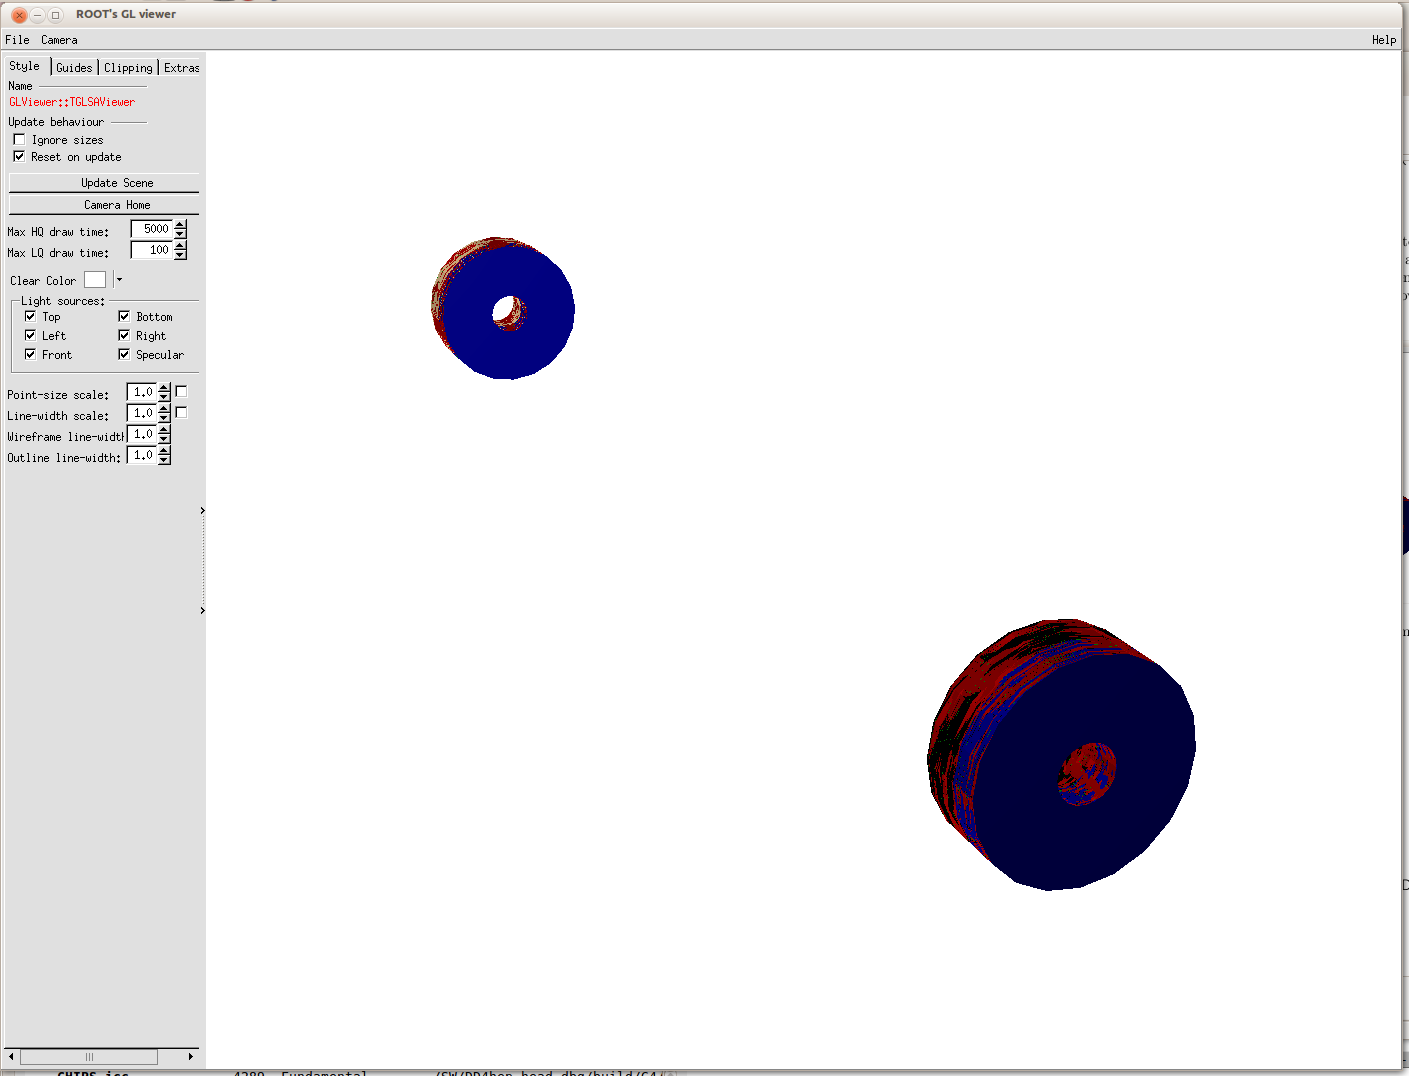
\includegraphics[width=80mm] {DD4hep-Lumical} &
      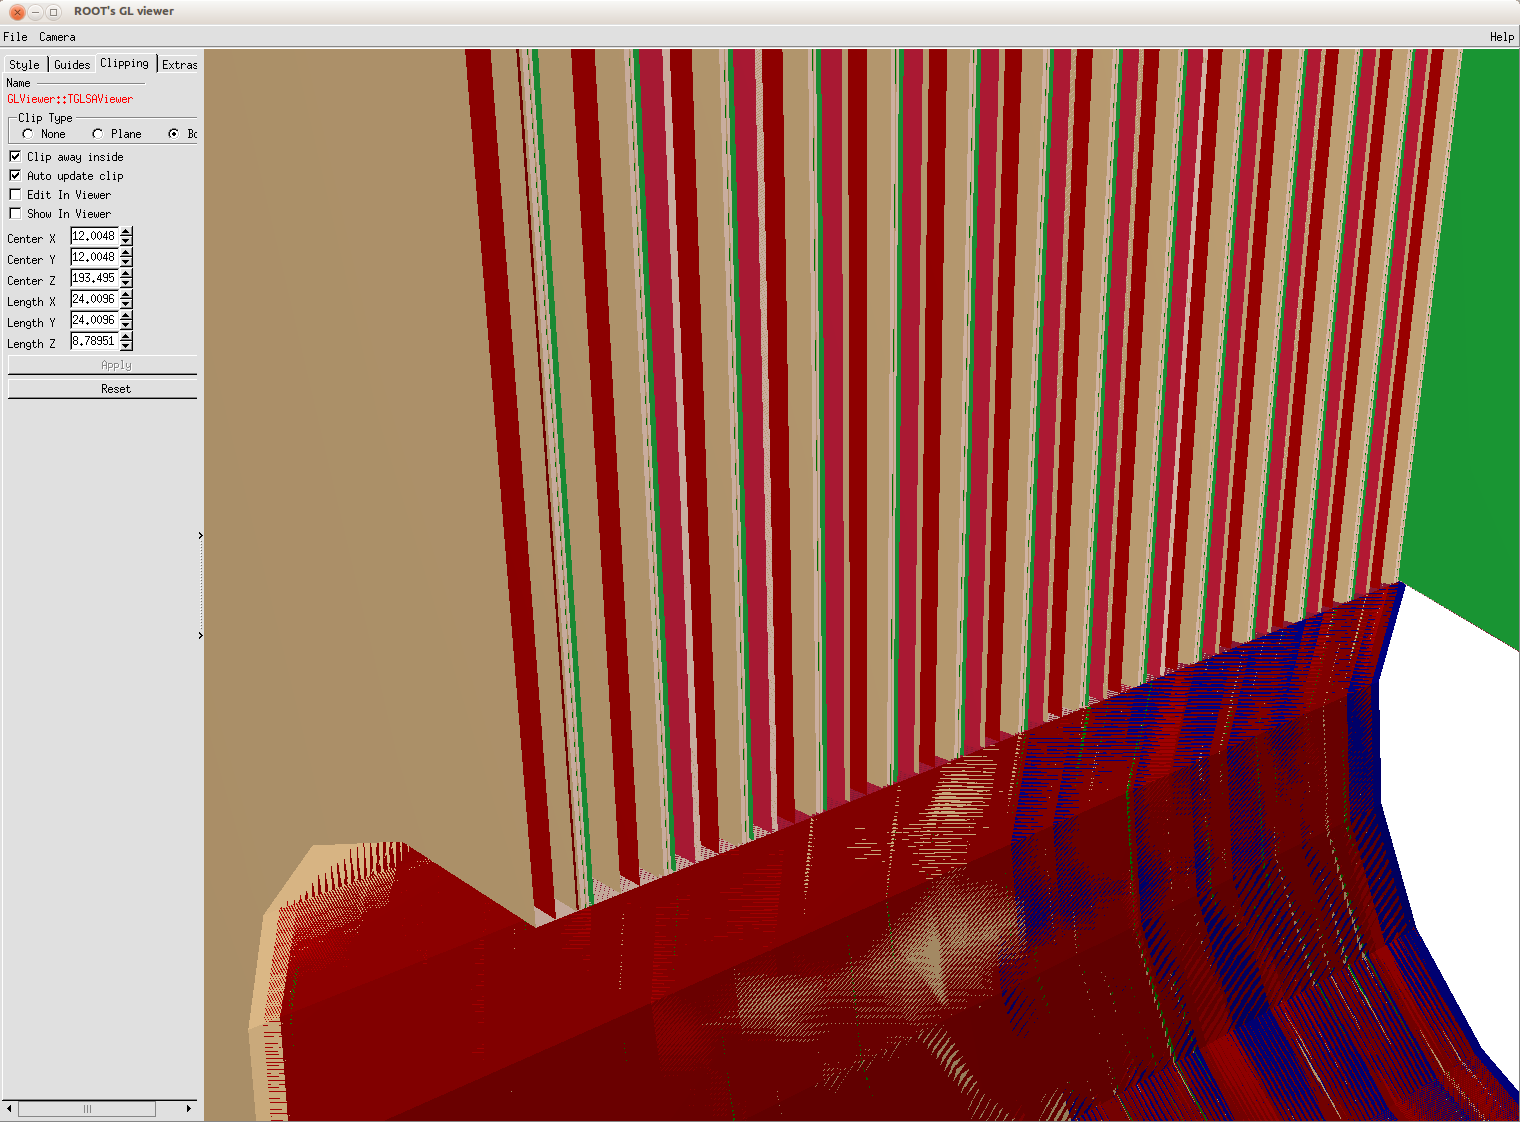
\includegraphics[width=80mm] {DD4hep-Lumical-detailed} \\
    \end{tabular}
    \caption{Geometry visualization using the ROOT OpenGL plugin.
        To the left the entire luminosity calorimeter is shown,
        at the right the detailed zoomed view with clipping to 
        access the internal layer and slice structure.}
    \label{fig:dd4hep-user-manual-visualization-subdetector}
  \end{center}
\end{figure}

The command to create the display is part of the DD4hep release:
\begin{minted}[frame=single,framesep=3pt,breaklines=true,tabsize=2,linenos,fontsize=\small]{bash}
$> geoDisplay -compact <path to the \texttt{XML} file containing the detector description>

 DD4hepGeometryDisplay -opt [-opt]                                                  
        -compact       <file>       Specify the compact geometry file              
                     [REQUIRED]     At least one compact geo file is required!     
        -build_type <number/string> Specify the build type                         
                     [OPTIONAL]     MUST come immediately after the -compact input.
                                    Default for each file is: BUILD_DEFAULT [=1]   
                                    Allowed values: BUILD_SIMU [=1], BUILD_RECO [=2] or BUILD_DISPLAY [=3]
        -destroy     [OPTIONAL]     Force destruction of the Detector instance         
                                    before exiting the application                 
        -volmgr      [OPTIONAL]     Load and populate phys.volume manager to       
                                    check the volume ids for duplicates etc.       
        -print      <number/string> Specify output level. Default: INFO(=3)        
                     [OPTIONAL]     Allowed values: VERBOSE(=1), DEBUG(=2),        
                                    INFO(=3), WARNING(=4), ERROR(=5), FATAL(=6)    
                                    The lower the level, the more printout...      
        -load_only   [OPTIONAL]     Dry-run to only load geometry without     
                                    starting the dispay.                      
\end{minted}


\subsection{Geometry Conversion}
\label{sec:dd4hep-manual-geometry-conversion}

\texttt{ROOT} \texttt{TGeo} is only one representation of a detector geometry. Other applications may require other representation. In particular two other are worth mentioning:
\begin{itemize}
\item \texttt{Detector}~\cite{Gaede:81331} the geometry representation used to simulate the ILC detector design with the \texttt{slic} application.
\item \texttt{GDML}~\cite{Chytracek:2006be} a geometry markup language understood by Geant4 and \texttt{ROOT}.
\end{itemize}
Both conversions are supported in DD4hep with the geoConverter application:
\begin{minted}[frame=single,framesep=3pt,breaklines=true,tabsize=2,linenos,fontsize=\small]{bash}
  geoConverter -opt [-opt]                                                
        Action flags:               Usage is exclusive, 1 required!           
        -compact2lcdd               Convert compact xml geometry to lcdd.     
        -compact2gdml               Convert compact xml geometry to gdml.     
        -compact2vis                Convert compact xml to visualisation attrs

        -input  <file>  [REQUIRED]  Specify input file.                       
        -output <file>  [OPTIONAL]  Specify output file.                      
                                    if no output file is specified, the output
                                    device is stdout.                         
        -ascii          [OPTIONAL]  Dump visualisation attrs in csv format.   
                                    [Only valid for -compact2vis]             
\end{minted}

\subsection{Overlap checking}
\label{sec:dd4hep-manual-overlap-checking}

Overlap checks are an important tool to verify the consistency of the  implemented geometrical design. As in the real world, where overlaps are  impossible, also simulated geometries may not have overlaps. In simulation overlaps tend to create particle reflections possibly leading to infinite loops.
\begin{minted}[frame=single,framesep=3pt,breaklines=true,tabsize=2,linenos,fontsize=\small]{bash}
    python <install>/DD4hep/bin/checkOverlaps.py --help
    Usage: checkOverlaps.py [options]

    Check TGeo geometries for overlaps.

    Options:
      -h, --help                        show this help message and exit
      -c <FILE>, --compact=<FILE>       Define LCCDD style compact xml input
      -p <boolean>, --print=<boolean>   Print overlap information to standard output
                                        (default:True)
      -q, --quiet                       Do not print (disable --print)
      -t <double number>, --tolerance=<double number>
                                        Overlap checking tolerance. Unit is in [mm].
                                        (default:0.1 mm)
      -o <string>, --option=<string>    Overlap checking option ('' or 's')
\end{minted}

\subsection{Geometry checking}
\label{sec:dd4hep-manual-geometry-checking}

Perform extensive geometry checks. For details and up to date information  please refer to the ROOT documentation of the class {\texttt{TGeoManager}}:
\begin{itemize}
\item Member function \texttt{TGeoManager::CheckGeometry} and 
\item Member function \texttt{TGeoManager::CheckGeometryFull}
\end{itemize}

\begin{minted}[frame=single,framesep=3pt,breaklines=true,tabsize=2,linenos,fontsize=\small]{bash}
    python <install>DD4hep/bin/checkGeometry.py --help
    Usage: checkGeometry.py [options]

    TGeo Geometry checking.

    Options:
      -h, --help                            show this help message and exit
      -c <FILE>, --compact=<FILE>           Define LCCDD style compact xml input
      -f <boolean>, --full=<boolean>        Full geometry checking
      -n <integer>, --ntracks=<integer>     Number of tracks [requires 'full']
      -x <double>, --vx=<double>            X-position of track origine vertex [requires 'full']
      -y <double>, --vy=<double>            Y-position of track origine vertex [requires 'full']
      -z <double>, --vz=<double>            Z-position of track origine vertex [requires 'full']
      -o <string>, --option=<string>        Geometry checking option default:ob
\end{minted}

The full geometry check performs the \texttt{TGeoManager:CheckGeometryFull} following actions:
\begin{itemize}
\item if option contains 'o': Optional overlap checkings (by sampling and by mesh).
\item if option contains 'b': Optional boundary crossing check + timing per volume.
\end{itemize}
\begin{description}
\item[STAGE 1] extensive overlap checking by sampling per volume. Stdout need to be checked by user to get report, then \texttt{TGeoVolume::CheckOverlaps(0.01, "s")} can be called for the suspicious volumes.
\item[STAGE 2] normal overlap checking using the shapes mesh - fills the list of overlaps.
\item[STAGE 3:] shooting NTRACKS rays from vertex \texttt{(vx,vy,vz)} and counting the total number of crossings per volume (rays propagated from boundary to boundary until geometry exit). Timing computed and results stored in a histogram.
\item[STAGE 4:] shooting 1 mil. random rays inside EACH volume and calling FindNextBoundary() + Safety() for each call. The timing is normalized by the number of crossings computed at stage 2 and presented as percentage. One can get a picture on which are the most ``burned'' volumes during transportation from geometry point of view. Another plot of the timing per volume vs. number of daughters is produced.
\end{description}

\subsection{Directional Material Scans}
\label{sec:dd4hep-manual-directional-material-scans}

Print the materials on a straight line between the two given points:
\begin{minted}[frame=single,framesep=3pt,breaklines=true,tabsize=2,linenos,fontsize=\small]{bash}
materialScan
 usage: print_materials compact.xml x0 y0 z0 x1 y1 z1 
        -> prints the materials on a straight line between the two given points ( unit is cm) 
\end{minted}
\texttt{materialScan} uses the python bindings provided by Geant4 and may be not  always availible. Alternatively the command \texttt{print\_materials} may be used, which does not use the python binding, but produces less pretty output.


\subsection{Plugin Test Program}
\label{sec:dd4hep-manual-plugin-test}

The plugin tester loads a given geometry and the executes a plugin defined at the command line. The main purpose of this program is to quickly  invoke new detector plugins while developing. The arguments for this  program are:
\begin{minted}[frame=single,framesep=3pt,breaklines=true,tabsize=2,linenos,fontsize=\small]{bash}
    geoPluginRun -opt [-opt]                                                
    
        -plugin <name>  [REQUIRED]  Plugin to be executed and applied.        
        -input  <file>  [OPTIONAL]  Specify geometry input file.              
        -build_type <number/string> Specify the build type                         
                     [OPTIONAL]     MUST come immediately after the -compact input.
                                    Default for each file is: BUILD_DEFAULT [=1]   
                                    Allowed values: BUILD_SIMU [=1], BUILD_RECO [=2] or BUILD_DISPLAY [=3]
        -destroy     [OPTIONAL]     Force destruction of the LCDD instance         
                                    before exiting the application                 
        -volmgr      [OPTIONAL]     Load and populate phys.volume manager to       
                                    check the volume ids for duplicates etc.       
        -print      <number/string> Specify output level. Default: INFO(=3)        
                     [OPTIONAL]     Allowed values: VERBOSE(=1), DEBUG(=2),        
                                    INFO(=3), WARNING(=4), ERROR(=5), FATAL(=6)    
                                    The lower the level, the more printout...
\end{minted}


\cleardoublepage
\phantomsection
\addreferencesline
\printbibliography

\end{document}
